%% SIMSON HEADER BEGIN
% POC: Fenella Saunders <fsaunders@sigmaxi.org>
%%
%% Special header designed for IEEE submissions
%%%

%
% This magic lets the Makefile create both the one-column version
% and the two-column version without the need to edit this file
%
\documentclass[11pt,letter]{article}
\usepackage[T1]{fontenc}        % http://tex.stackexchange.com/questions/664/why-should-i-use-usepackaget1fonte
\usepackage[utf8x]{inputenc}	% accented letters in tex files allowed
\usepackage{ucs}                        % more unicode support
\usepackage{fancyvrb}
\usepackage[margin=1in]{geometry}
\usepackage{graphics}
\usepackage{marvosym}
\usepackage{amsmath}
% \usepackage{unicode}
% \usepackage{textcomp}
\usepackage{listings}
\usepackage{tabularx}
\usepackage{euro}
\usepackage{tabularx}           % tables that expand to with width requested
\usepackage{titletoc}		% adds toc commands
\usepackage{titlesec}		% complete replacement for titles
\usepackage{fancyhdr}		% puts chapters names in footers
\usepackage{ccaption}		% control captions
\usepackage{setspace}           % enabled \doublespacing, \onehalfspacing, etc.
\usepackage{multicol}           % multiple columns; good for you!
\usepackage{fancyvrb}           % a better verbatim
\usepackage{varioref}		% provides \vref - smart referencing
\usepackage{xspace}             % provides \xspace
\usepackage{nps_sf298}           % Bring in SF298 for the documentation page
\usepackage{latexsym}           % gives \Box
\usepackage{graphicx}           % it's better
\usepackage{multirow}           % for table cells with multiple row   
\usepackage{pifont}             % fancy characters
\usepackage{remreset}           % prevent footnotes from being reset at each chapter
\usepackage{color}
\usepackage{xcolor}
\usepackage{paralist}           % {compactenum} {compactitem} environments
\usepackage{enumitem}		% No extra space before lists
\usepackage{float}                  % reimplementation of float package
\usepackage{cite}                   % for [5-8] reference style
\usepackage{amsmath}                % for many types of math equations
\usepackage{url}		    % nice handling of URLs
\usepackage{times}


\newcommand{\wikipedia}[1]{See \url{#1}}
\newcommand{\wikipediab}[1]{ and \url{#1}}

%\usepackage{xspace}             % optional spaces
%\usepackage{graphicx}           % better graphics importing
\usepackage{url}                % make \url work and link
%\usepackage{fancyvrb}           % a fancy verbatim
%\usepackage{fancyhdr}
%\usepackage{paralist}           % gives compactitem, etc.
%\usepackage{listings}           % source code listings
%\usepackage{tabularx}           % the ``X'' for tables
%\usepackage{pifont}             % symbols
%\usepackage{color}              % some people like commenting in color
\DefineShortVerb{\|}            % makes |foo| a verbatim command

% Change control
%\usepackage[today,revrange,fancyhdr,margin]{svninfo}                % include subversion info
\usepackage{svn}
\SVNdate $Date$


% Useful cross-reference commands
\newcommand{\Sref}[1]{\S\ref{#1}}
\newcommand{\chapref}[1]{Chapter~\ref{#1}\xspace}
\newcommand{\chapvref}[1]{Chapter~\vref{#1}\xspace}
\newcommand{\figref}[1]{Figure~\ref{#1}\xspace}
\newcommand{\secref}[1]{Section~\ref{#1}\xspace}
\newcommand{\secvref}[1]{Section~\vref{#1}\xspace}
\newcommand{\figvref}[1]{Figure~\vref{#1}\xspace}
\newcommand{\tabref}[1]{Table~\ref{#1}\xspace}
\newcommand{\tabvref}[1]{Table~\vref{#1}\xspace}
\newcommand{\appref}[1]{Appendix~\ref{#1}\xspace}
\newcommand{\appvref}[1]{Appendix~\vref{#1}\xspace}

% Useful symbols and abbreviations
%\newcommand{\checkmark}{\Pisymbol{pzd}{52}}
\newcommand{\naive}{na\"{\i}ve\xspace}
\newcommand{\etc}{\emph{etc.}\xspace}
\newcommand{\eg}{\emph{e.g.\ }}
\newcommand{\etal}{\emph{et al.\ }}

% Try not to float graphics to their own pages
\renewcommand{\topfraction}{0.99}
\renewcommand{\floatpagefraction}{0.99}

% \sgraphic[optional width=8in]{filename}{caption}
% Then use \figref{filename} to get a reference to the figure
\newcommand{\sgraphic}[3][width=\linewidth]{
  \begin{figure}
  \begin{center}
  \fbox{\includegraphics[#1]{#2}}
  \end{center}
  \caption{#3\label{#2}}
  \end{figure}
}

% \sgraphicb[optional width=8in]{filename}{caption}
% \sgraphicb is like sgraphic, but may put it at the bottom of the page
\newcommand{\sgraphicb}[3][width=\linewidth]{
  \begin{figure}
  \begin{center}
  \fbox{\includegraphics[#1]{#2}}
  \end{center}
  \caption{#3\label{#2}}
  \end{figure}
}

% \sgraphicn[optional width=8in]{filename}{caption}
% \sgraphicn is like sgraphic, but does not put a box around the graphic
\newcommand{\sgraphicn}[3][width=\textwidth]{
  \begin{figure}
  \begin{center}
  \includegraphics[#1]{#2}
  \end{center}
  \caption{#3\label{#2}}
  \end{figure}
}

% \sgraphico[optional width=8in]{filename}{caption}
% \sgraphico is like sgraphic, but it doesn't create a figure
\newcommand{\sgraphico}[3][width=\textwidth]{
  \begin{center}
  \fbox{\includegraphics[#1]{#2}}
  \end{center}
%  \caption{#3\label{#2}}
}

% \sgraphicon[optional width=8in]{filename}{caption}
\newcommand{\sgraphicon}[3][width=\textwidth]{
  \begin{center}
  \includegraphics[#1]{#2}
  \end{center}
%  \caption{#3\label{#2}}
}

%% SIMSON HEADER END

\newcommand{\be}{\textit{bulk\_extractor}\xspace}

\newcommand{\citeN}[1]{\cite{#1}}

\begin{document}
\title{The Science of Digital Forensics Research}
\author{Simson L.\ Garfinkel}
\maketitle
\pagenumbering{arabic}


% Special commands for the American Scientist article
% 

\newcommand{\chapter}[1]{}
\renewcommand{\section}[1]{\noindent\textbf{\textsc{#1}}}
\renewcommand{\subsection}[1]{\noindent\textbf{#1}}
\newcommand{\citep}[1]{\nocite{#1}}
\newcommand{\citet}[1]{\nocite{#1}}
\renewcommand{\cite}[1]{\nocite{#1}}



%% Comments from editor: 

%% At the end of the piece, there is not really a strong conclusion to
%% finish your narrative. Do you think you could add a sentence or two
%% that would sum things up a bit? Something about the current state of
%% the field, what's up and coming, why things might be looking up, etc?
%% Perhaps something about the fact that there will always be an arms
%% race between criminals and investigators, but new tools hope to make
%% it possible for law enforcement to stay a step ahead? 
%% 
%% Let me know what you think. I'm happy to help in any way possible.
%% 
%% 

\chapter{Introduction}
Over the past decade \emph{digital forensics} (DF) has grown from a trade
practiced by technicians working for law enforcement
organizations and into scientific discipline. Today DF  researchers are
making slow but steady progress on scientifically challenging
problems; DF research is presented at conferences
and published in peer-reviewed journals; and there is a growing
collection of both tools and reference data sets designed to promote
DF education and help validate new research techniques. Because of
both the scale and the diversity of their domain, DF researchers and
practitioners are necessarily at the forefront of some of the most
challenging problems in computer science today, including ``big data''
analysis, natural language processing, visualizations, and
cybersecurity. This article introduces the science of DF research
to those who are not acquainted with the field. 

Broadly construed, DF applies the process and goals of \emph{forensic
  science} to the study of all things digital---and specifically to
digitized information that might be found on computers, cell phones,
storage devices and  computer networks during the course of a
criminal investigation. Compared with traditional ``blood and
bullets'' forensics, DF poses significant challenges for three primary
reasons: information on a computer system can be changed without 
trace; the scale of data that must be analyzed; and the variety of
data types that an investigator can encounter. Just as a traditional forensic investigator must be
prepared to analyze any kind of smear or fragment, no matter the
source, a DF investigator must be able to make sense of any data that
might be found on any digital device anywhere on the planet. In
practice, this is a very difficult proposition.

Much of what we now call DF got its start in the 1980s
as computer systems were increasingly involved in criminal acts.
From its inception, DF served two different
purposes. First, in many cases computers contained evidence of a
crime. In these cases the crime took place in the physical world
and the computer was all but incidental---except for the fact that
computerization made the evidence harder for
investigators to analyze than paper records. For example, Bernard Madoff kept track of
his victims ``accounts'' using an IBM AS/400 minicomputer from the
1980s: the age of the computer  helped perpetuate the crime, since few
people on Wall Street have experience with 25-year-old technology, and
was an added complication to investigators after Madoff was
arrested\cite{technology-madoff}, since investigators had few tools
necessarily to make sense of the data.

The second class of cases are those in
which the crime was inherently one involving computer systems, such as
computer hacking. In these cases, investigators are hampered
by the technical sophistication of the systems and the massive amount
of evidence to analyze.

Today personal computers have become so
ubiquitous that the collection and use of computerized evidence is no
longer a curiosity---it is now a part of many criminal and civil
investigations. Suspects in murder cases now routinely have their
laptops and cell phones examined for corroborating evidence---not
because a computer was the instrument of the crime, but because
computers now mediate so many human-human interactions. 
E-discovery dominates much of today's corporate litigation.

DF is powerful because computer systems are windows into the
past. Many digital systems retain vast quantities of
information---either intentionally, in the form of log files and
archives, or inadvertently, as a result of software that does not
cleanly erase memory and files after it runs. As a result, it
is frequently possible for investigators to recover old email
messages, chat logs,   Google search terms and other kinds of data
that were created
weeks, months, or even years in the past. Such contemporaneous records
can reveal an individual's state-of-mind or intent \emph{at the time
  the crime was being committed}.

But whereas pre-computer evidence such as handwritten letters and
photographs could be photographically reproduced and given to attorneys, judges and juries, computerized evidence
requires special handling and analysis. In part this is because
electronic data are easily changed, damaged or erased if
handled improperly---for example, simply turning on a consumer GPS
may cause the device to erase critical evidence. Additionally,  computers
frequently harbor hidden evidence that may only be evident when
specialized tools are used---for example, a digital camera may appear to have
30 photos, but examination by an expert may reveal that another 300
deleted photos can be recovered.

Because they can look into the past and uncover hidden data,
DF tools are increasingly used beyond the courtroom. Security
professionals use DF tools to analyze network intrusions---not
to convict the attacker, but to understand how the
attacker gained access to plug the hole. Data recovery firms use DF tools to resurrect files from drives that have
been inadvertently formatted or damaged. DF tools can even 
detect the  unintentional disclosures of personal information---for
example, by analyzing computers at the conclusion of a lease to see if
sensitive information remains on their hard drives. For example, in
2009 the Inspector General of the United States Department of Defense
issued a report in which forensic software was used to test hard
drives leaving the government service. The IG found that ``DOD Components did not properly
sanitize, document, or fully account for excess unclassified IT
equipment before it was released to other Federal, DOD, or non-Federal
organizations.''\cite{D-2009-104}

Forensic tools are also used to determine that something did not
happen. Here they are less powerful, for the well known reason that
the absence of evidence is not the evidence of absence. 
For example, in May 2006 a laptop and external hard drive containing
sensitive personal information of 26.5 million veterans and military
personnel was stolen from an employee at the Department of Veterans
Affairs. After the stolen laptop was recovered in June 2006, forensic
investigators analyzed the media and determined that the sensitive
files had probably not been accessed\cite{va-laptop-1}. One way to
make such a determination is by examining the access and modification
times associated with each file on the computer's hard
drive. Of course, the same
forensic techniques that the investigators used could have been
applied to access the VA laptop without modifying those timestamps,
the VA investigators really just determined that the files had not
been asked by convention, non-forensic means.

As the preceding paragraphs make clear, today the field of digital
forensics is largely \emph{tool-based} and
\emph{investigator-centric}. 
That is, the requirements of DF are driven 
by what investigators need to perform digital
investigations\citep{walls-levine-effective-digital-forensics}. Convictions
are frequently the
measure of success. In many cases there is a considerable gap between
what is theoretically possible and what is necessary. That is, even
though there may be an intellectual desire to analyze and explain every last byte
on a piece of subject media\cite{garfinkel:every-last-byte}, there is
rarely a reason to do so.

\section{The Digital Forensics Process and Toolbox}

The tools of digital forensics can be equally applied to suspects,
victims and bystanders. A cell phone found on a dead body without
identification would almost certainly be subjected to analysis, but so
would a phone dropped during a house burglary. For this reason,
discussions of techniques speak about systems under investigation in
abstract terms (e.g. the ``subject computer''). Discussions of
legal issues such as the need for a warrant are separated from
discussions of technology, because different techniques are
permissible in different legal contexts.

Variations in use and policy can be challenging. As the field has
grown, practitioners have tried to create a consistent approach for
performing DF investigation, but the approach must be flexible enough
to cover these different applications. Today we call this approach the
\emph{digital forensic model}. Several such models have been
proposed\citep{pollitt:models}, but most have these common elements:


% http://www.tex.ac.uk/cgi-bin/texfaq2html?label=complist
\subsection{Preparation} 
Before an individual or organization
  performs an investigation, it's important to decide upon the
  standards and procedures that will be followed; to obtain the
  appropriate devices, software, and even cables required for investigations; and to assure that
  investigators and technicians are appropriately trained. In some
  cases preparation may take years, requiring 
  certification of forensic laboratories and the formal testing of
  tools to determine their effectiveness and error rates. 

  When it comes to preparation, two important tools are the American Society of Crime Laboratory
  Directors/Laboratory Accreditation Board (ASCLD/LAB) laboratory
  accreditation program and individual examiner certification programs such as
  the Certified Computer Examiner.

\subsection{Collection and Preservation} 
Before data can be analyzed, they
  are taken from the field (the ``scene of the crime''),
  stabilized and preserved to create a lasting record. 

  Although digital computers are based entirely on computations
  involving the binary digits 0 and 1, more commonly known as
  \emph{bits}, modern computers do most of their work on groups of
  eight bits called \emph{bytes}. Because each binary digit can be a 0
  or a 1, a byte can represent the numbers $00000000$, $00000001$,
  $00000010$, $\ldots$ $11111111$, or the decimal numbers 0 through
  255 (recall that $2^8=256$). When working with digital forensics,
  it's common to use hexadecimal representation (base 16), which
  represents these are the numbers \texttt{00} through \texttt{FF}
  ($15\times16+15=255$).

  One common use for bytes inside the computer is to store written
  text. To store text, each letter is represented by a specific binary
  code. UTF-8, a common representation in use today, uses the
  binary sequence 00100001 (hexdecimal \texttt{41}) to represent the
  letter A, 00100010 (\texttt{42}) for the letter
  B. 
\includegraphics{uni/unicode_547d} is the Han ideograph
  representing life; it has the hexdecimal coding \texttt{547D}. 

When recorded on a hard drive or camera card, these bytes are groups in
  blocks called \emph{sectors} that are typically 512 or 4096 bytes in
  length. A sector is the smallest block of data that a drive can read
  or write. An email message might require 10 or 20 sectors to
  store; a movie might require hundreds of thousands. Depending on the
  arrangement of other files on the device, the sectors can be stored
  as a single sequential stream or they can be fragmented into many
  different locations. Other sectors contain information that the
  computer uses to find the stored information: such bookkeeping
  information is called ``file system metadata.''

  Each sector on the disk has a unique identifying number, called
  the sector's \emph{logical block address} (LBA). An Android phone
  advertised as having ``8GB'' of storage has eight billion bytes or roughly 15
  million sectors.  To preserve the data on a computer or phone, each of these sectors
  must be individually copied out of the phone or off the hard drive and
  stored on another computer in a single file called a \emph{disk image}
  or \emph{physical image}. This file, which contains every single byte
  stored on the target device, naturally includes every
  visible file on the media. But the physical image also records
  invisible files as well as portions of files that have been deleted
  but not yet overwritten by the operating system. 

  For typical desktop or laptop computers, collection and preservation
  is performed with a program called a \emph{disk imager}, of which there
  are many. Disk imager  are tested by the Computer Forensic
  Tool Testing Program (CFTTP) at the National Institute of Standards and
  Technology (NIST) Information Technology Lab (ITL) to make sure that
  they accurately copy all of the data off the subject
  device. Although it might seem straightforward, the task is
  complicated by the possible presence of bad sectors and ``hidden''
  storage, the need for the program to detect and accurately report
  the drive being unplugged, and other issues that may seem
  inconsequential but which can be very significant when a disk image
  is being used as the basis of a criminal prosecution. 

  In the case of network forensics, it is the actual data
  sent over the network connection that are preserved. This means that network forensics
  equivalent to a wiretap---and in fact network forensics equipment is
  increasingly used for wiretaps by law enforcement. 

%  Today's computer networks carry information in blocks
%  called \emph{packets} which are typically between 50 and 1500 bytes
%  in length. Network collection is performed with tools called
%  \emph{packet sniffers} or \emph{network forensic analysis tools}
%  (NFATs)\cite{613756}. These tools intercept the packets that are
%  sent down a wire (or through the air) and copy them into a file
%  called a ``packet trace'' or a ``PCAP'' (packet capture) file.  

  Increasingly the random access memory (RAM) associated with computer
  systems is also being subjected to forensic investigation. RAM is
  difficult to work with, as it changes very quickly and is lost when
  a computer is turned off. RAM must also be captured with a special
  program (a ``memory imager'') and is stored in its own special kind
  of file called a ``memory dump.'' Although memory can be extracted from all
  kinds of computer systems, including desktops, laptops, cell phones,
  as well as network communications equipment such as wireless
  routers, each of these systems uses different kinds of internal
  structures, so software designed to analyze one may not analyze another.

  Although forensics researchers have developed approaches for
  assuring the forensic integrity of drive copies, currently there is
  no widely accepted approach for mathematically assuring a RAM dump.

\subsection{Examination and Extraction} Working with the preserved data, an
  examiner will explore for any information that might be
  relevant to the investigation at hand. 

  When performing disk forensics, files that can be seen from within
  the computer's own operating system are called ``allocated files''
  because the storage associated with the files is allocated to that
  purpose. On many system it is also possible to recover files that have
  been deleted but whose previously allocated sectors have not yet
  been overwritten or otherwise used for another purpose. These
  sectors are said to contain \emph{deleted files}, \emph{residual data}, or
  \emph{digital trace evidence}.

Most examinations are performed
  with tools that can extract user files from the disk image, search for files that contain a specific word or phrase
  in a variety of human languages, and even detect the presence of
  encrypted data. One common technique is to arrange all of the
  information chronologically and create a timeline that shows when
  each file on the disk was modified or last accessed. Another 
  technique is to review every directory and file and look for
  things that seem out-of-the-ordinary. Relevant data are then
  extracted from the preserved system so that they are easier to
  analyze---for example, an individual file may be sent to a linguist
  for translation. In the military this process of examination and extraction
  is frequently called \emph{exploitation}.

  There are many tools for performing examination. The Sleuth Kit\cite{sleuthkit} is
  an open source tool that can decode Windows, Macintosh, Linux, XBox,
  and Android
  file systems, recovering both allocated and deleted
  files;   Volatility\cite{volatility} can analyzing memory dumps from a
  variety of different systems.

\subsection{Analysis} Once potentially relevant information is
  extracted, an analyst will construct one or more hypotheses that
  uses the digital evidence to explain possible past activities. A
  hypothesis may draw from multiple digital devices---an email message
  sent from a desktop computer to a cell phone, for example---or the
  hypothesis may incorporate events in the physical world, like a
  power failure or theft. During this phase a good analyst will also
  try to construct alternative hypotheses that are consistent with the
  evidence but which point to different conclusions. In Europe it is
  popular for examiners to perform an Bayesian analysis and estimate
  the probability of each hypothesis based on the available data.

  Many examination tools can perform some kind of analysis, but there
  are also commercial tools that specialize at this task. Examples
  include Analyst Notebook\cite{analysts_notebook} and
  Palantir\cite{palantir}, as well as general purpose tools such as
  Microsoft Excel.

\subsection{Reporting and Testimony} Finally, the analyst will
  produce a written report or give testimony in a courtroom. Remember,
  judges and juries can't examine digital evidence for
  themselves---even if they had the training and the technical skills
  to do so, performing their own analysis would be inappropriate:
  their role in the legal process is to evaluate the law, the evidence
  and make a legal determination, not to perform technical
  analysis. Reports and testimony must be
  \emph{complete}---they must describe the tools and procedures
  that were followed, clearly document what was found, and then
  separately provide the technical interpretation of the
  evidence. (For this very reason, Rule 704 of the US Federal Rules of
  Evidence, allow a DF expert to
  express an opinion on ``an ultimate issue to be decided by the trier
  of fact'' in most circumstances.)

  Not surprisingly, the most common reporting tools are traditional
  office automation programs such as Microsoft Word and PowerPoint. 

\section{The Science of Technical Exploitation}

In the early 1990s there were no DF tools as we know them
today. Instead practitioners had to repurpose tools that had been
developed for other purposes. For example, backup software was
used for collection and preservation, while data recovery tools were used
for examining subject media. Although these approaches worked, they lacked control,
repeatability, and a known error rates---that is, examiners had no way
of knowing the accuracy of their results. 

In 1993 the US Supreme Court held in the case of Daubert v. Merrell
Pharmaceutical 
that any scientific testimony presented in court must be based on a theory
that is testable; that has been scrutinized and found favorable by the
scientific community; that has a known or potential error rate; and
that is generally accepted\cite{daubert}. This case didn't directly
kick off the demand for DF tools, but it did give DF practitioners
grounds for arguing that validated tools were needed not just as a matter
of good science and procedure, but as a matter of law. 

Since then there has been a steady development of techniques and the
incorporation of those techniques in a variety of tools. This section
presents several techniques for what has come to be called
\emph{technical exploitation}. The first two techniques---hashing and
file extraction---now dominate all DF processing. The next three
techniques---reconstruction of compressed data, memory parsing, and
fraud detection in multimedia---represent the next generation of DF
research that is leveraging new algorithms and signal processing
approaches to help address challenges facing DF practitioners today.

\subsection{Hashing}

Probably the single most transformative technical innovation in
DF has been the introduction of hash functions, first as a means for assuring the integrity of forensic data,
and later as a way to recognize specific files.

In computer science a \emph{hash function} is any function that maps a
sequence of zero or more characters (called a \emph{string}) to an
binary number of a specific fixed size---that is, a fixed number of
bits. A 16-bit hash
function can produce $2^{16}=65,536$ different hash values, while a
32-bit hash function can produce $2^{32}=4,294,967,296$ possible hash
values. Hash functions are designed so that changing a single
character in the input results in a completely different number. While
the pigeonhole principle guarantees that many different strings will
have the same hash value---something that's called a \emph{hash
  collision}---the more bits in the hash has, the smaller the chance
of a collision.

Hashing was invented by H.\ P.\ Luhn in a 1953 IBM technical memo;
it's been widely used for computerized text processing since the
1960s. For example, because every sentence in a document can be
treated as a string, hashing makes it possible to rapidly see if the
same paragraph ever repeats in a long document: just computer the hash
value for each paragraph, put all of the hashes into a list, sort the
list, and see if any number repeats twice. If there is no repeat, then
no paragraph is repeated. Of course, if a number \emph{does} repeat,
then it's necessary to look at the paragraphs that correspond to those
two numbers to determine if the same paragraph really is repeated
twice or the duplicate is the result of a hash collision. Using hashes
in this manner is much faster than working directly with the
paragraphs because it is much faster for computers to compare numbers
than sequences of words---even when you take into account the time to
perform the hashing.

(Interesting fact: The name \emph{hash} comes from the way hash functions are typically
implemented as a two-step process that first chops and then mixes the
data, much in the way that one might make hash in the kitchen!)

In 1979 Stanford University PhD student Ralph Merkle invented a way to use
hashing for computer security\citep{merkle:79}. Merkle's idea was to
use a hash
function that produced more than 100 bits of output and that
additionally had the property of being \emph{one-way}. That is, it was
a function for which it was relatively easy to compute the hash of a
string, but it was nearly impossible, given a hash, to find a
corresponding string. The essence of Merkle's idea was to use a
document's 100-bit one-way hash as a stand-in for the document itself
for certain mathematical purposes. For example, instead of digitally
certifying a 50-page document, the document could be reduced to a
100-bit hash and the hash could then be certified. Because there are so many different possible hash values
($2^{100}\approx10^{30}$), Merkle reasoned that it would not be
possible for an attacker to take the digital signature from one document and use it
to certify a second document---because to do so would require that
both documents had the same hash value.

Merkle got his PhD, and today digital signatures applied to hashes are
the basis of many cyber security system. Digital signatures protect
credit card numbers sent over the Internet, certify the authenticity
and integrity of code run on iPhones, and validate keys used play
digital music. The idea of hashing has been applied to other areas as
well---in particular, forensics.

One of the first and continuing uses of hashing in DF was to establish
\emph{chain-of-custody} for forensic data. Instead of hashing a
document or a file, the hash function is applied to the entire disk
image---that is, \emph{all} of the bytes extracted from a hard
drive. Many law enforcement organizations will create two
disk images of a drive and then computer the hash of each image.  If the values match, then the
copies are assumed to each be a true copy of the data that were on the
drive. The hash value is then included in the official report. With
the hash recorded, the image file can be copied to a server at the
police department, to an investigator's workstation, or even given to
a forensic expert working for the other side. Any investigator with the
data can calculate the hash and see if it matches the original
reported value. If the hashes match, the investigator can be sure that
not a single bit in the disk image has been changed since the original
image was recorded. Hashing is so important that many DF tools can
automatically validate an evidence file by recomputing the hash and
comparing it with a stored value.

A second use for hashing is to identify specific
files. This approach takes advantage of the property that it is
extraordinarily unlikely for two files to have the same
hash value. File hashes can thus be used to identify files in much the
same way that a person can be identified by their fingerprints. 

Today forensic practitioners distribute databases containing the file
hashes as a standard part of forensic processing. The best known of these data
sets is the National Software Reference Library Reference Data Set,
distributed by the National Institute of Standards and
Technology\cite{nist-nsrl-rds-march2012}. These data sets can be used
to identify \emph{known goods}, such as programs distributed as part
of operating systems, or \emph{known bads} such as computer viruses,
stolen documents and child of pornography. Recent work is now
applying cryptographic hashing to blocks of data smaller than
files\cite{garfinkel:sector-id}, taking advantage of the fact that
even relatively short 512-byte and 4096-byte segments taken from
files can be highly identifying. 

File and sector identification with hashing means that a hard drive
containing millions of files can be automatically searched against a
database containing the hashes of hundreds of millions of file hashes
in a relatively short amount of time---perhaps just a few hours. Importantly, the search can be done without any human
intervention.

\subsection{Files Recovery and File carving}

Many forensic investigations start with the examiner looking for
files belonging to the computer's previous user. But what is a file?

On modern digital systems, a \emph{file} is a sequence of
\emph{bytes}. Files therefore
have \emph{contents} and a \emph{length}, but they do not necessarily have other
information that computer users typically associate with files, such
as a \emph{file name} or a \emph{modification date}. These attributes
are called \emph{metadata} (literally ``data about data'')
and are stored by the computer's \emph{file system}, but are not
strictly part of the file. (Some operating systems even allow a single
file to have multiple names or timestamps, further complicating the
issue.)

\emph{Allocated files} are files that can be viewed
through the file system and whose contents will not under normal
circumstances be inadvertently overwritten by the operating
system. The word ``allocated'' refers to the \emph{disk sectors} in
which the file's content is stored. The sectors are allocated in the
sense that they are dedicated to the file and cannot be assigned to
other files and overwritten. Allocated files are present in either the
file system's \emph{root directory} or a \emph{sub directory}. These
are the files that a user typically sees with the Windows Explorer or
the Apple Finder. Many DF tools allow the examiner to see allocated
files present in a disk image without having to use the computer's
native operating system. This makes it possible to maintain forensic
integrity of the evidence.

One of the major technical DF innovations of the
past 15 years has been approaches for
recovering a file after it is deleted. These are not simply files that are in
a ``trash can'' or ``recycle bin''---these are the files after the
trash has been emptied. So-called \emph{deleted files} can be
recovered because many operating systems don't actually overwrite the
sectors of files when the user deletes them. Instead, the file names
are hidden and the storage associated with the files is
\emph{deallocated}. Similar techniques can also be used to
recover deleted email messages in Microsoft Outlook ``\texttt{.pst}'' files.

Sometimes a file's content remains on the computer's hard
drive, in memory, or on external media but the metadata that could be
used to recover the deleted file is overwritten or otherwise lost. Recovering
these kinds of data requires a technique called \emph{file carving}.

File carving appears to have been invented by independent security researcher
Dan Farmer and was incorporated into the first open source digital
forensics tool called The Coroner's Toolkit written and released by Farmer and IBM
researcher Wietse Venema in 1999. Two years later 
the United
States Air Force Office of Special Investigations released a file carver called Foremost, developed by Kris Kendall and
Jesse Kornblum. Today one of the most powerful file carvers is 
a tool called PhotoRec, developed by Christophe Grenier, a computer
security specialist in France. A common use
of these tools is to recover images from digital camera memory cards
that have been accidentally formatted.

File carvers take advantage of the fact that the internal structure of
many file types contain
characteristic sequences of bytes at the beginning and
end  of each file. Such sequences are called \emph{file headers} and
\emph{footers}. For example, JPEG files generated by
most digital cameras typically begin with the hexadecimal sequence \texttt{FF D8 FF E0} and end
\texttt{FF D9}  (numbers that can be determined by examining a large
number of JPEGs or by reading the JPEG standard). The file carver simply scans the disk image for JPEG
headers and footers. When a header and matching footer are found, the
two sequences of bytes, and all of the data between them, are saved in
a new file on the analyst's workstation.

Today more than a dozen file carvers have been developed that can
run on Windows, Macintosh and Linux computers. Modern carvers can
validate the data that they are carving (for example, to make sure
that the bytes between the JPEG header and footer can be actually
displayed as a digital photograph), and can even reassemble files that are fragmented
into multiple pieces\citep{pal-sht}. Fragment recovery carving is
computationally challenging because the number of ways that fragments
can be combined: the result is a combinatorial explosion as the size of
the media increases. Missing fragments further complicates the problem.

File carving is an incredibly powerful technique. It can recover files
from any kind of computer system---even those that were unknown when
the carver was created---and it works even when a portion of media is
damaged and unreadable. But file carving typically cannot recover the
\emph{name} of a file, and it frequently finds information that is
unrelated to the case at hand.


\subsection{Reconstruction of compressed data}

Closely related to file carving is the problem of reconstructing
compressed data. \emph{Compression} is a technique that is widely used
on computer systems to squeeze data so that it takes less space than
it otherwise would. Compression exploits redundancy; for example,
asked to compress the character sequence ``humble humbleness,'' a computer might
replace the characters the second set of the six characters ``humble''
with a pointer to the first occurrence. Compressed English text typically
takes a sixth its original size.

Text must be compressed with \emph{lossless} algorithms that
faithfully restore the original text when the compressed data is
decompressed. Photographs and Video is
typically compressed with \emph{lossy} systems that exploit
deficiencies in the human perceptual system when they decompress. For
example, a few dozen pixels of slightly different colors might
be replaced by a single rectangle of uniform hue. The resulting
savings can be immense. Without compression an hour of
full-screen video might require 99 gigabytes\footnote{30 screens of
  640x480 video per second with 3 bytes per pixel}, but with
compression the same video might require only 500 megabytes---roughly
$\frac{1}{200}^\textrm{th}$ the original size. 

The primary challenge posed by compression is recovering data when the
compressed file is corrupted or partially missing. Just five years ago
such corruption frequently made it impossible to recover anything of
use. But lately there has been dramatic advances in this area. In 2009
Professors Husrev Sencar from TOBB University of Economics and
Technology and Nasir Memon from NYU Poly developed an approach that
can be used to show a fragment of a JPEG digital photograph even if
the beginning and end of the file is missing\cite{jpeg-recovery}. And
in 2011 Ralf Brown from CMU developed an approach for recovering data
from fragments of files compressed with the ZIP or DEFLATE
algorithm\cite{dfrws2011:RalfBrown}. The algorithm is particularly
impressive because critical information needed for reassembly is
missing. Brown's approach creates a model of the many different ways
that a document might decompressed based on the underlying
mathematics, then chooses between the different possible documents
based on a second model of the human language in which the document is
written (Figures \ref{brown-1} through \ref{brown-4}).

\begin{figure}
\begin{tabular}{p{3.2in}|p{3.2in}}
\hline
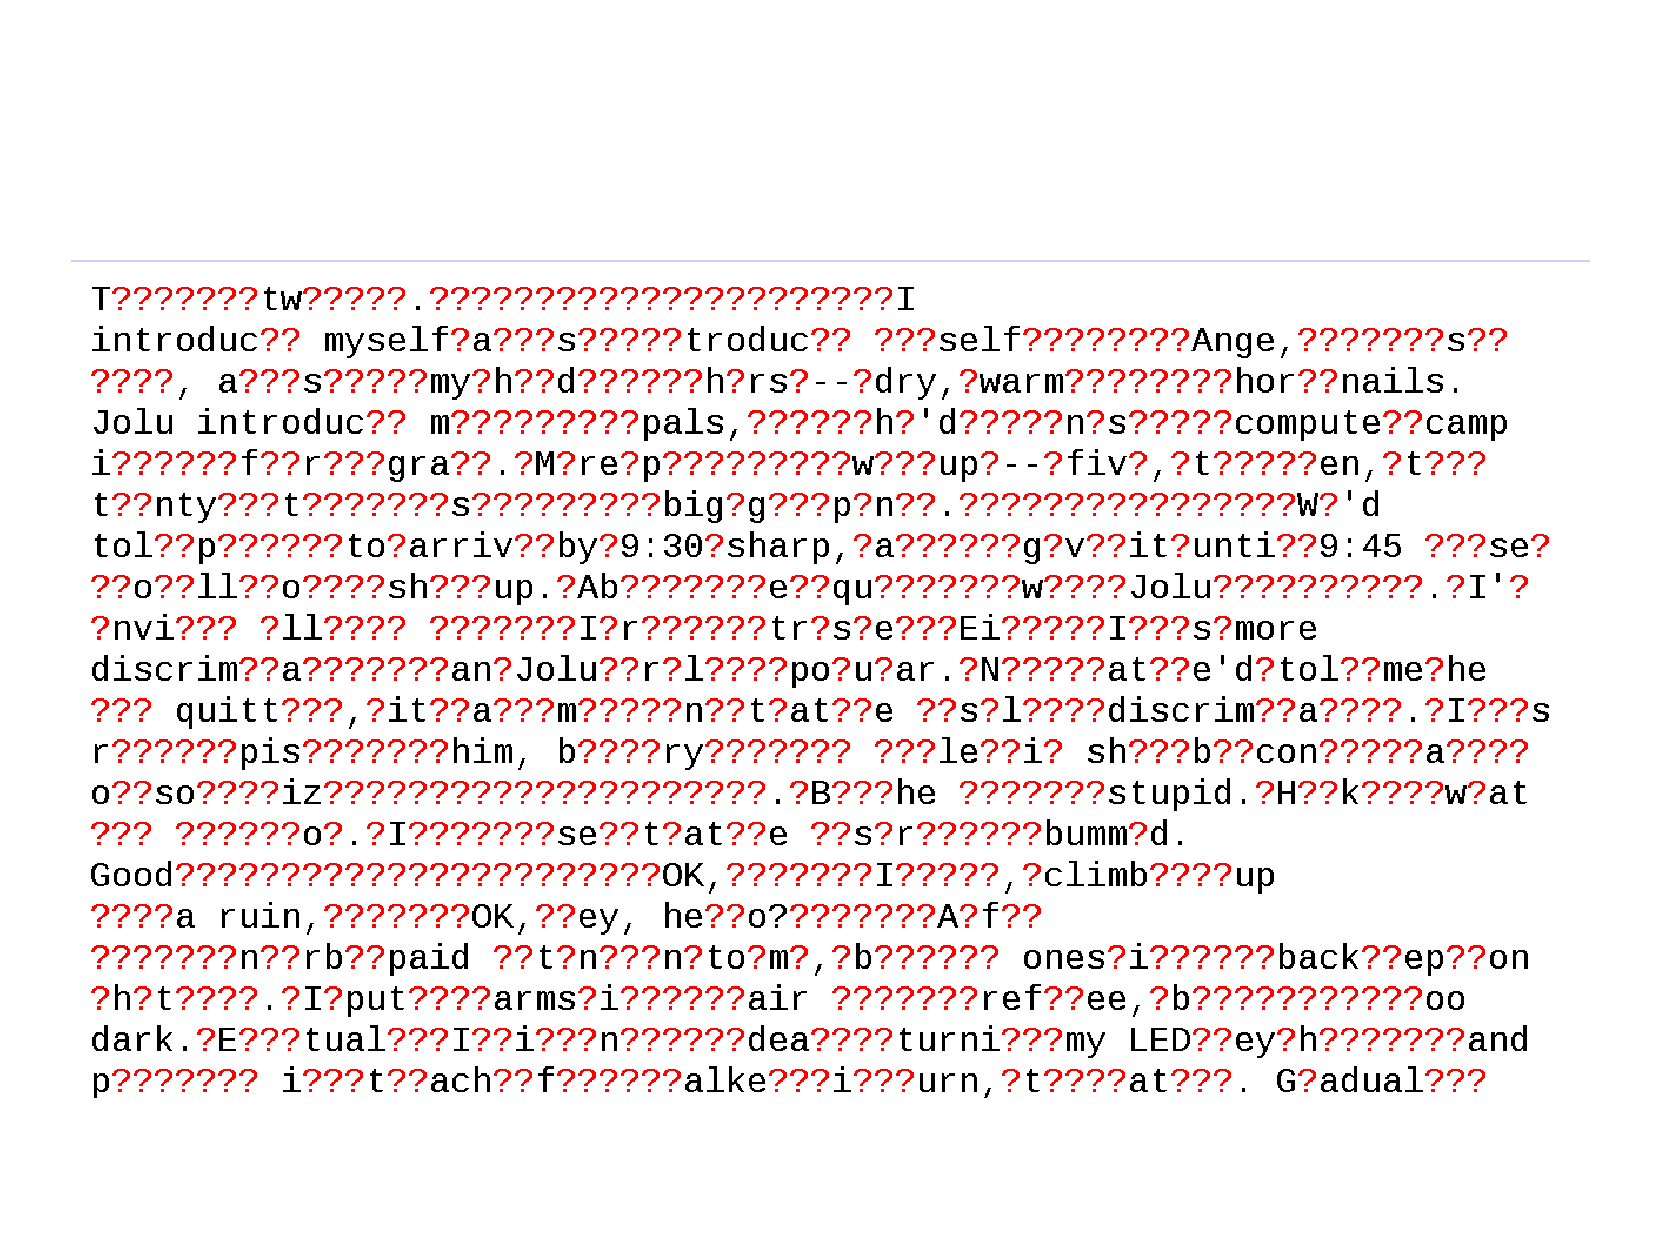
\includegraphics[width=3in]{art/brown-1} &  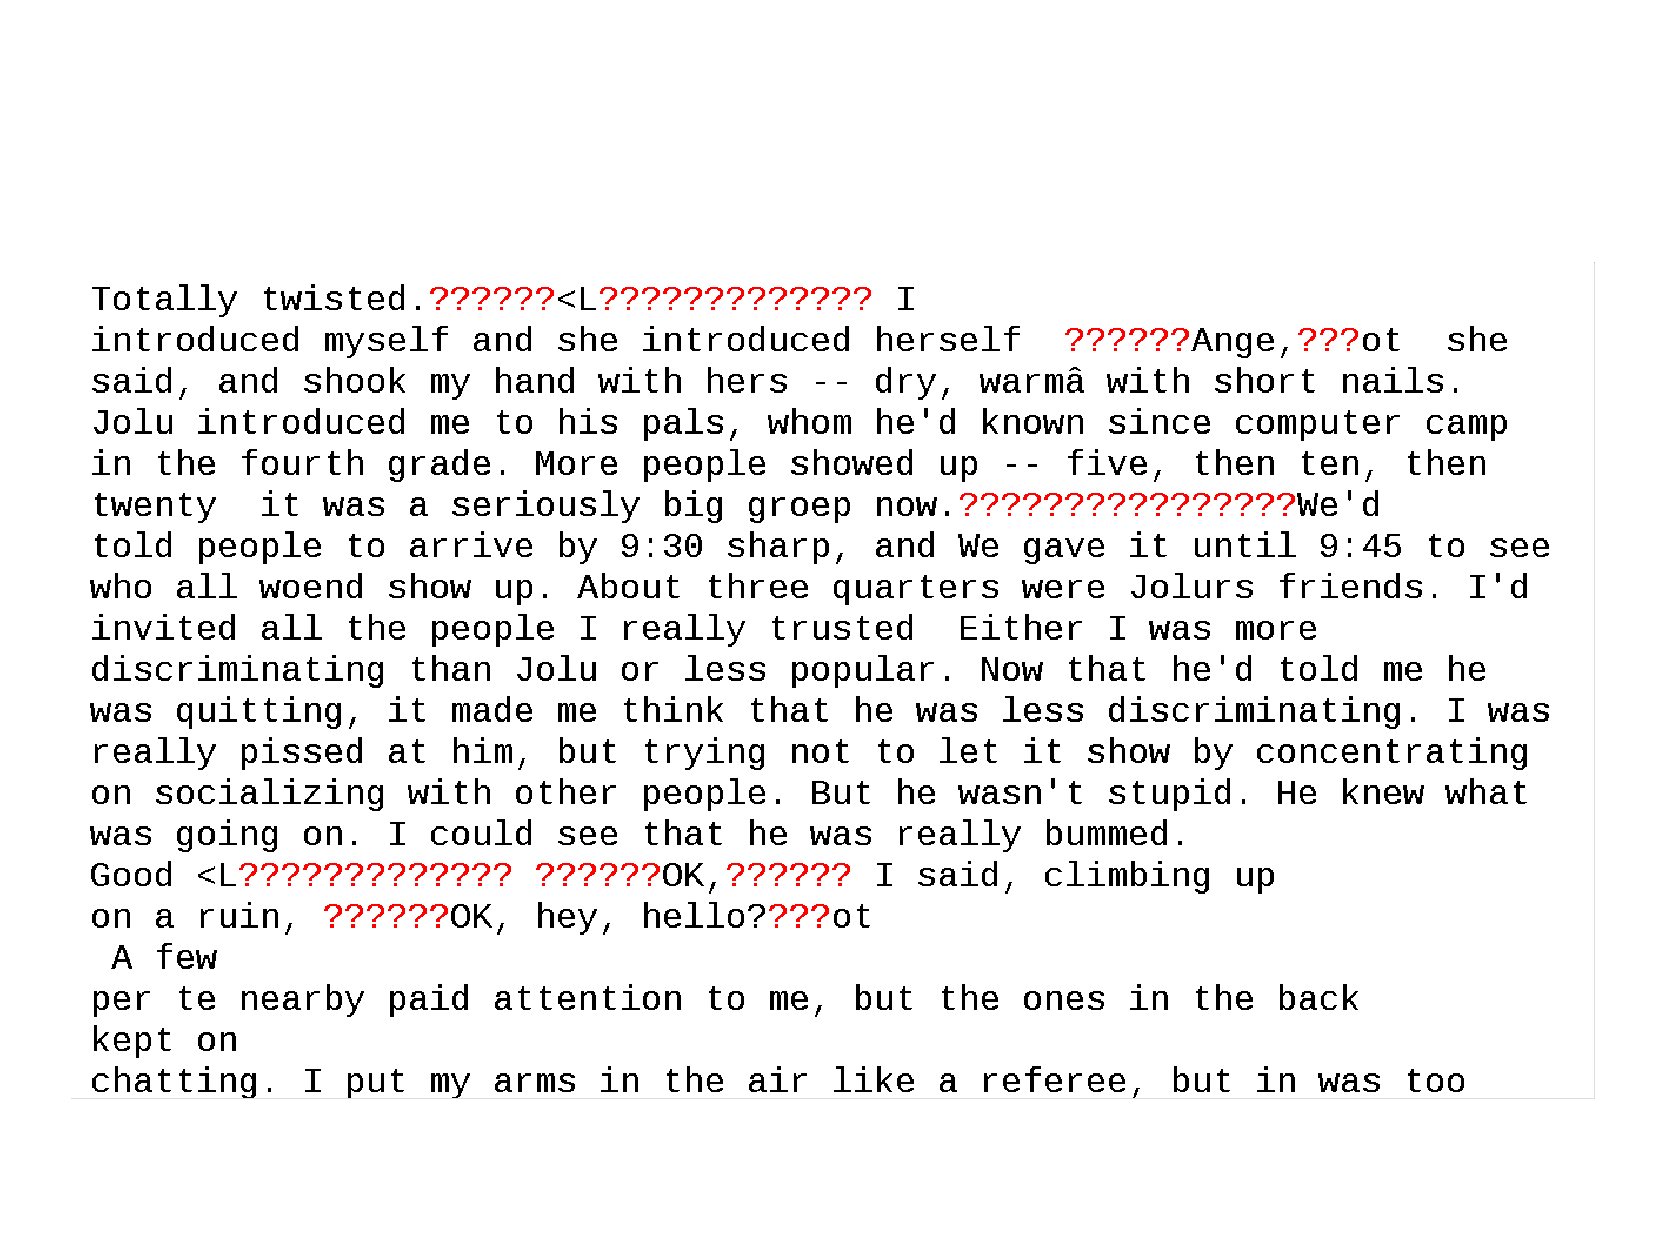
\includegraphics[width=3in]{art/brown-2} \\
\caption{Reconstructed text, without language model}\label{brown-1}
& \caption{Best possible reconstructed text, with language model}\label{brown-2}\\
\hline
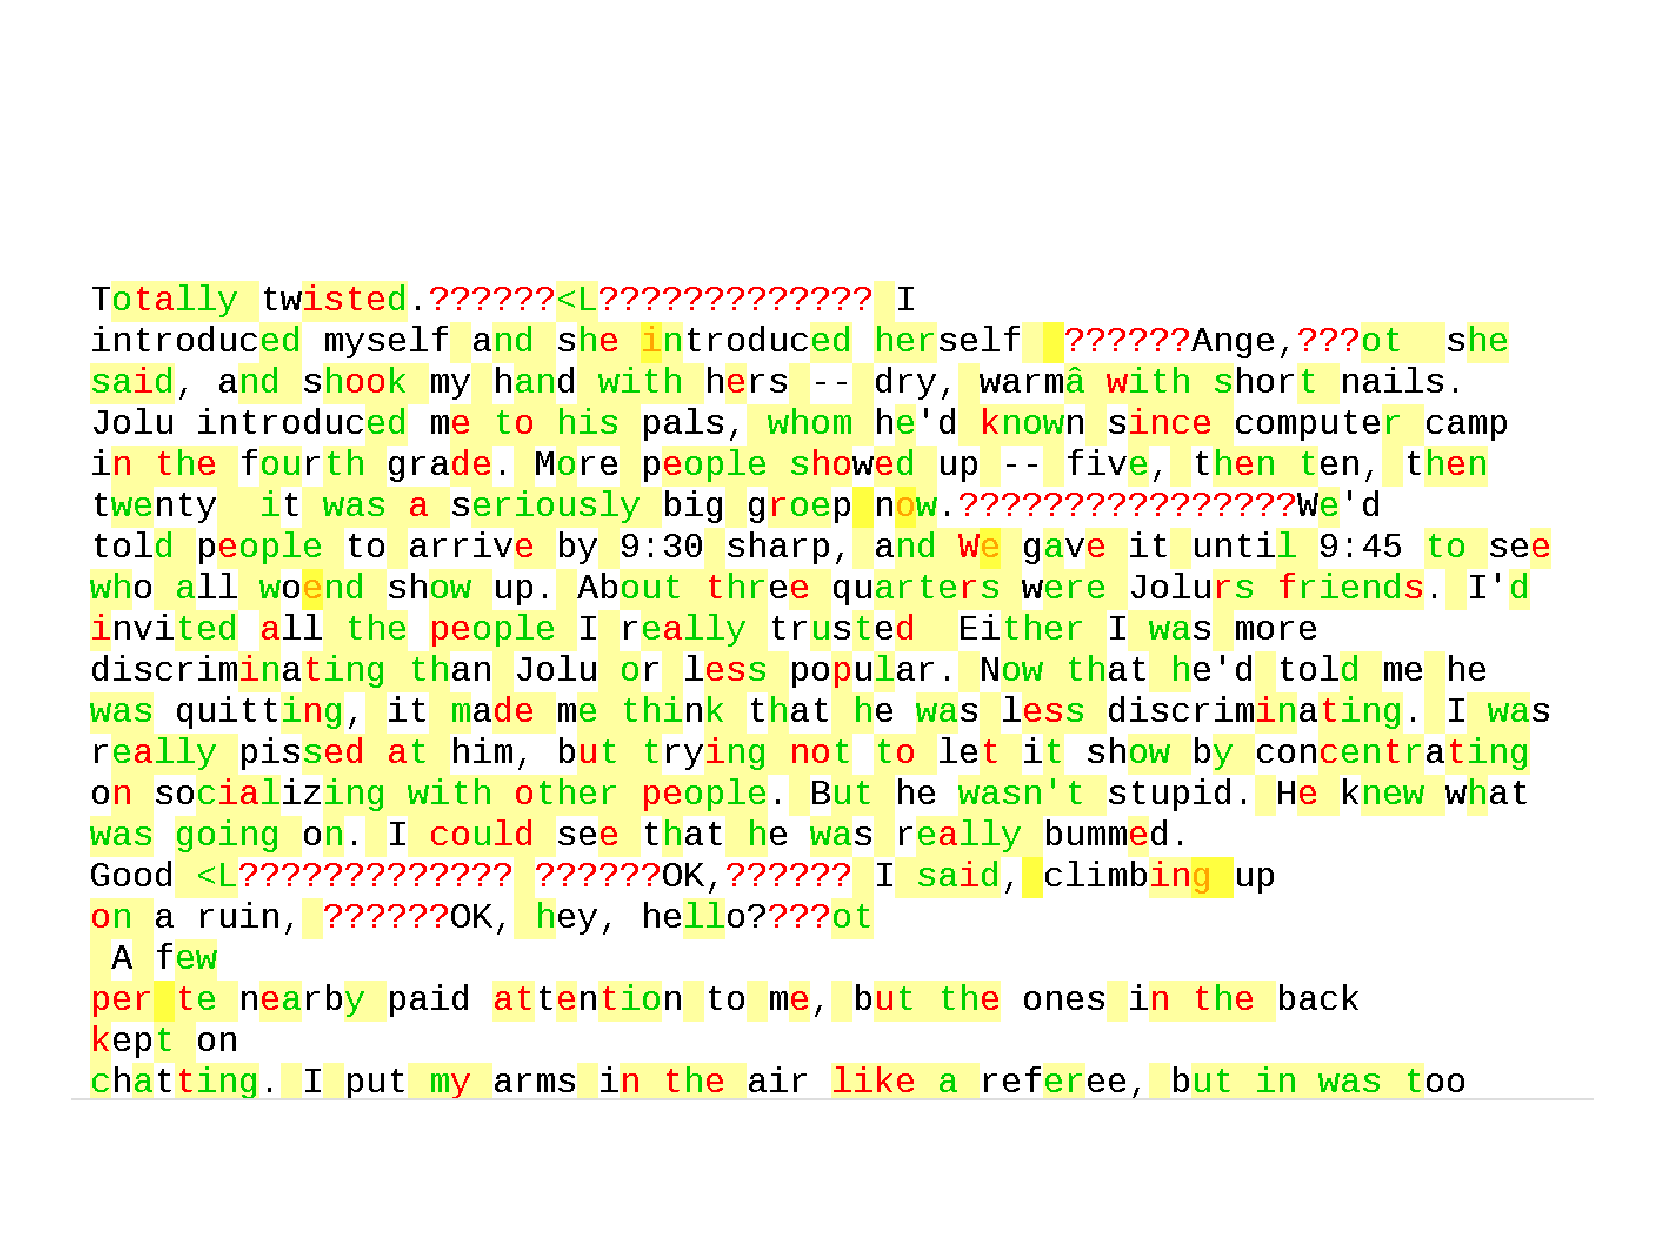
\includegraphics[width=3in]{art/brown-3} & 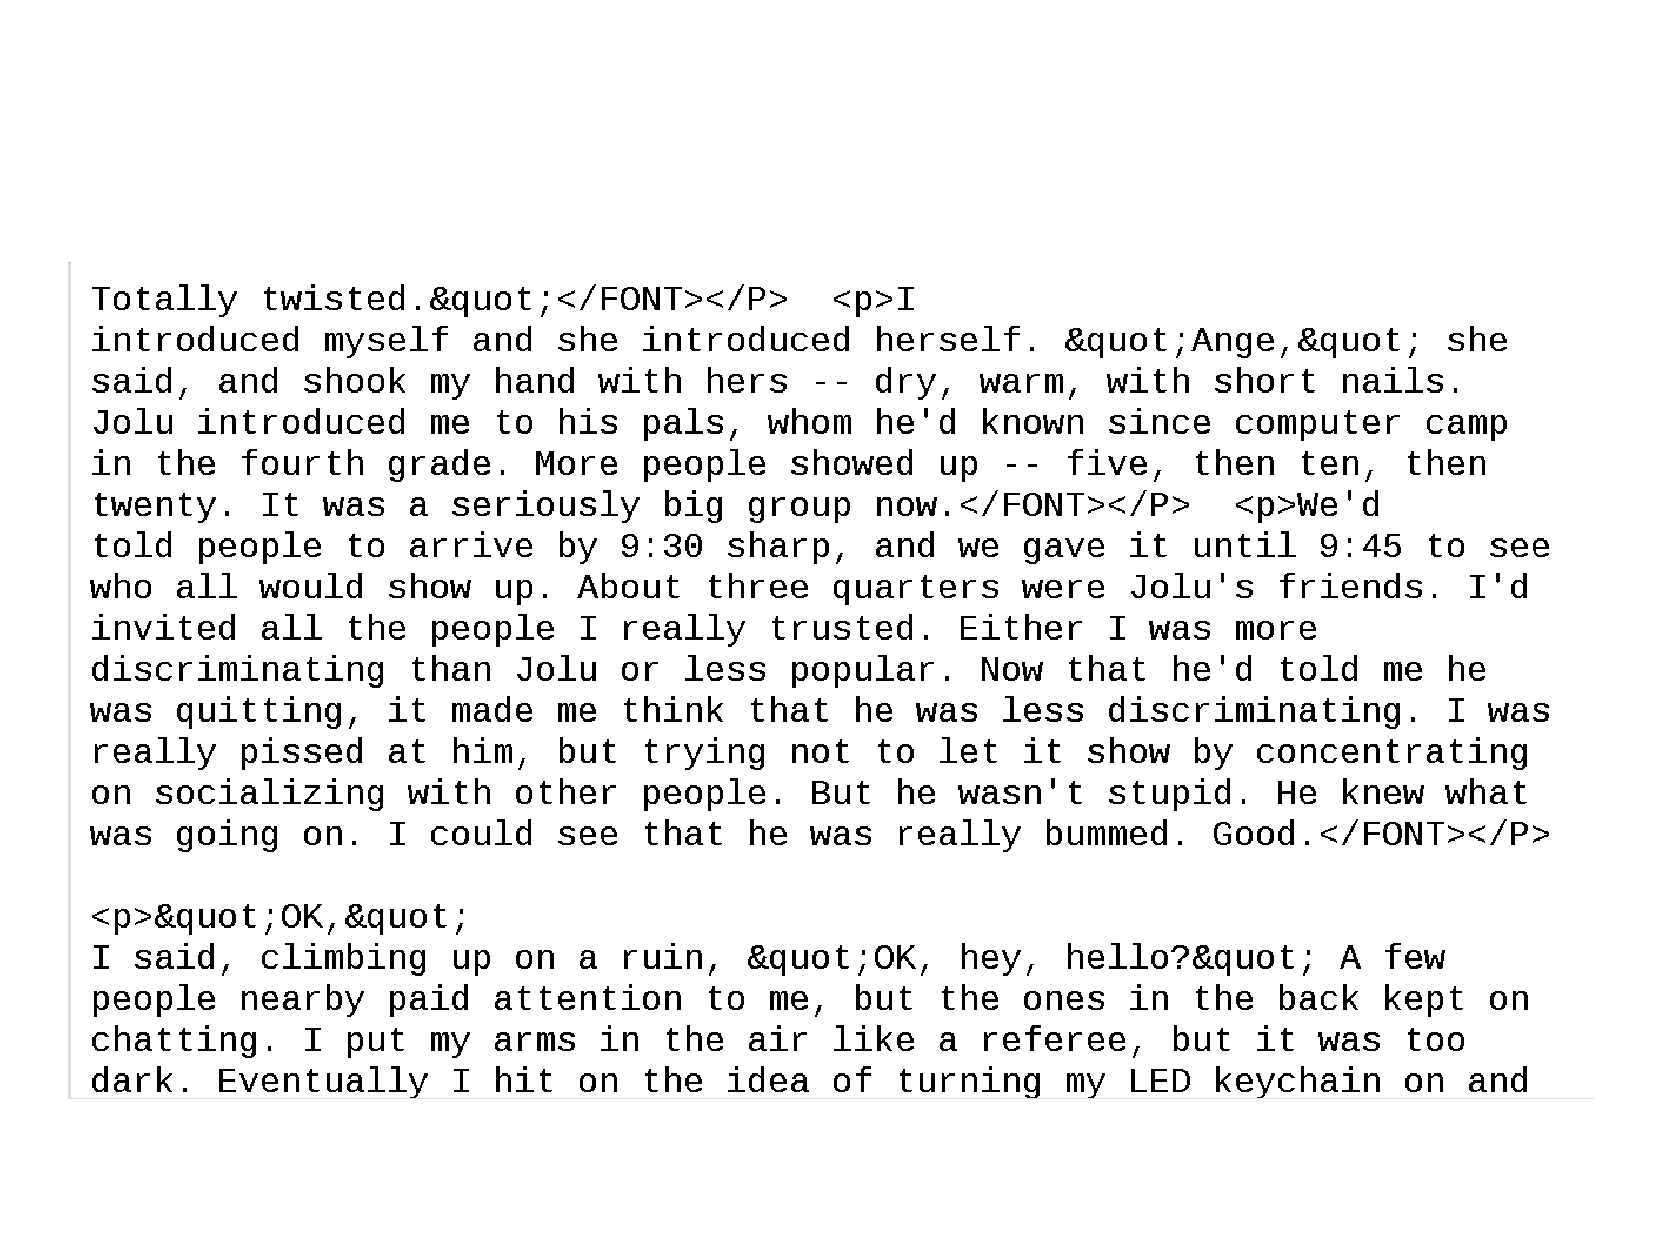
\includegraphics[width=3in]{art/brown-4}\\
\caption{Best possible reconstructed text, with language model. Green
  letters indicate high-probability matches, red letters indicate
  low-probability matches.}\label{brown-3}
&
\caption{Original text, from HTML version of Cory Doctorow novel
  ``Little Brother'', compressed using Info-Zip version 3.0, first
  1024 bytes of archive removed}\label{brown-4}
\\
\hline
\end{tabular}
\end{figure}


\subsection{Memory Parsing}

The memory of a desktop, laptop or cell phone is a mosaic of 4096-byte
blocks that variously 
contain running program code,  fragments of programs
that recently ran and have exited, portions of the computer's
operating system, fragments of what was sent and received over the
network, fragments of windows displayed on the computer's screen, the
computer's copy-and-paste buffer, and other kinds of information. Memory
changes rapidly---typical memory systems support several billion
changes per second---so it is nearly impossible to make a copy that is
internally consistent without halting the machine. An added complication is that the very
specific manner that programs store information in memory is rarely
documented and changes between one version of a program and
another. As a result, each version may need to be painstakingly reverse-engineered by
computer forensics researchers. Thus, memory analysis is time consuming, very
difficult, and necessarily incomplete.

Despite these challenges, recent years has seen the development of
forensically sound techniques for acquiring and analyzing the contents
of a running computer system. Today there are both open source and
proprietary memory analysis tools. These tools can take a memory dump
and report the system time when the memory was captured, display a
list of running processes, open files, and even display the contents
of the computer's clipboard and screen. Today memory analysis tools
are widely used for reverse-engineering computer viruses, worms and
other kinds of \emph{malware}, as well as for understanding an
attacker's actions in computer intrusion cases. Memory analysis can be combined
with carving to recover digital photographs and video.

\subsection{Fraud Detection in Multimedia}

Even when photos and video can be recovered from a subject's computer
or cell phone, another question to consider is whether or not the
imagery is real. Photographs were doctored long before the advent of
PhotoShop. For example, after he was purged by Stalin, Abel
Yenukidze was carefully removed from official photographs through a
series of skillful manipulations of light and negatives in a Kremlin darkroom\citet{stalins-darkroom}. Today
computer animation takes such manipulation to a completely new level,
with computers now able to synthesize scenes that are 
indistinguishable from recorded reality (\figref{ultra-realistic}). 

\begin{figure}
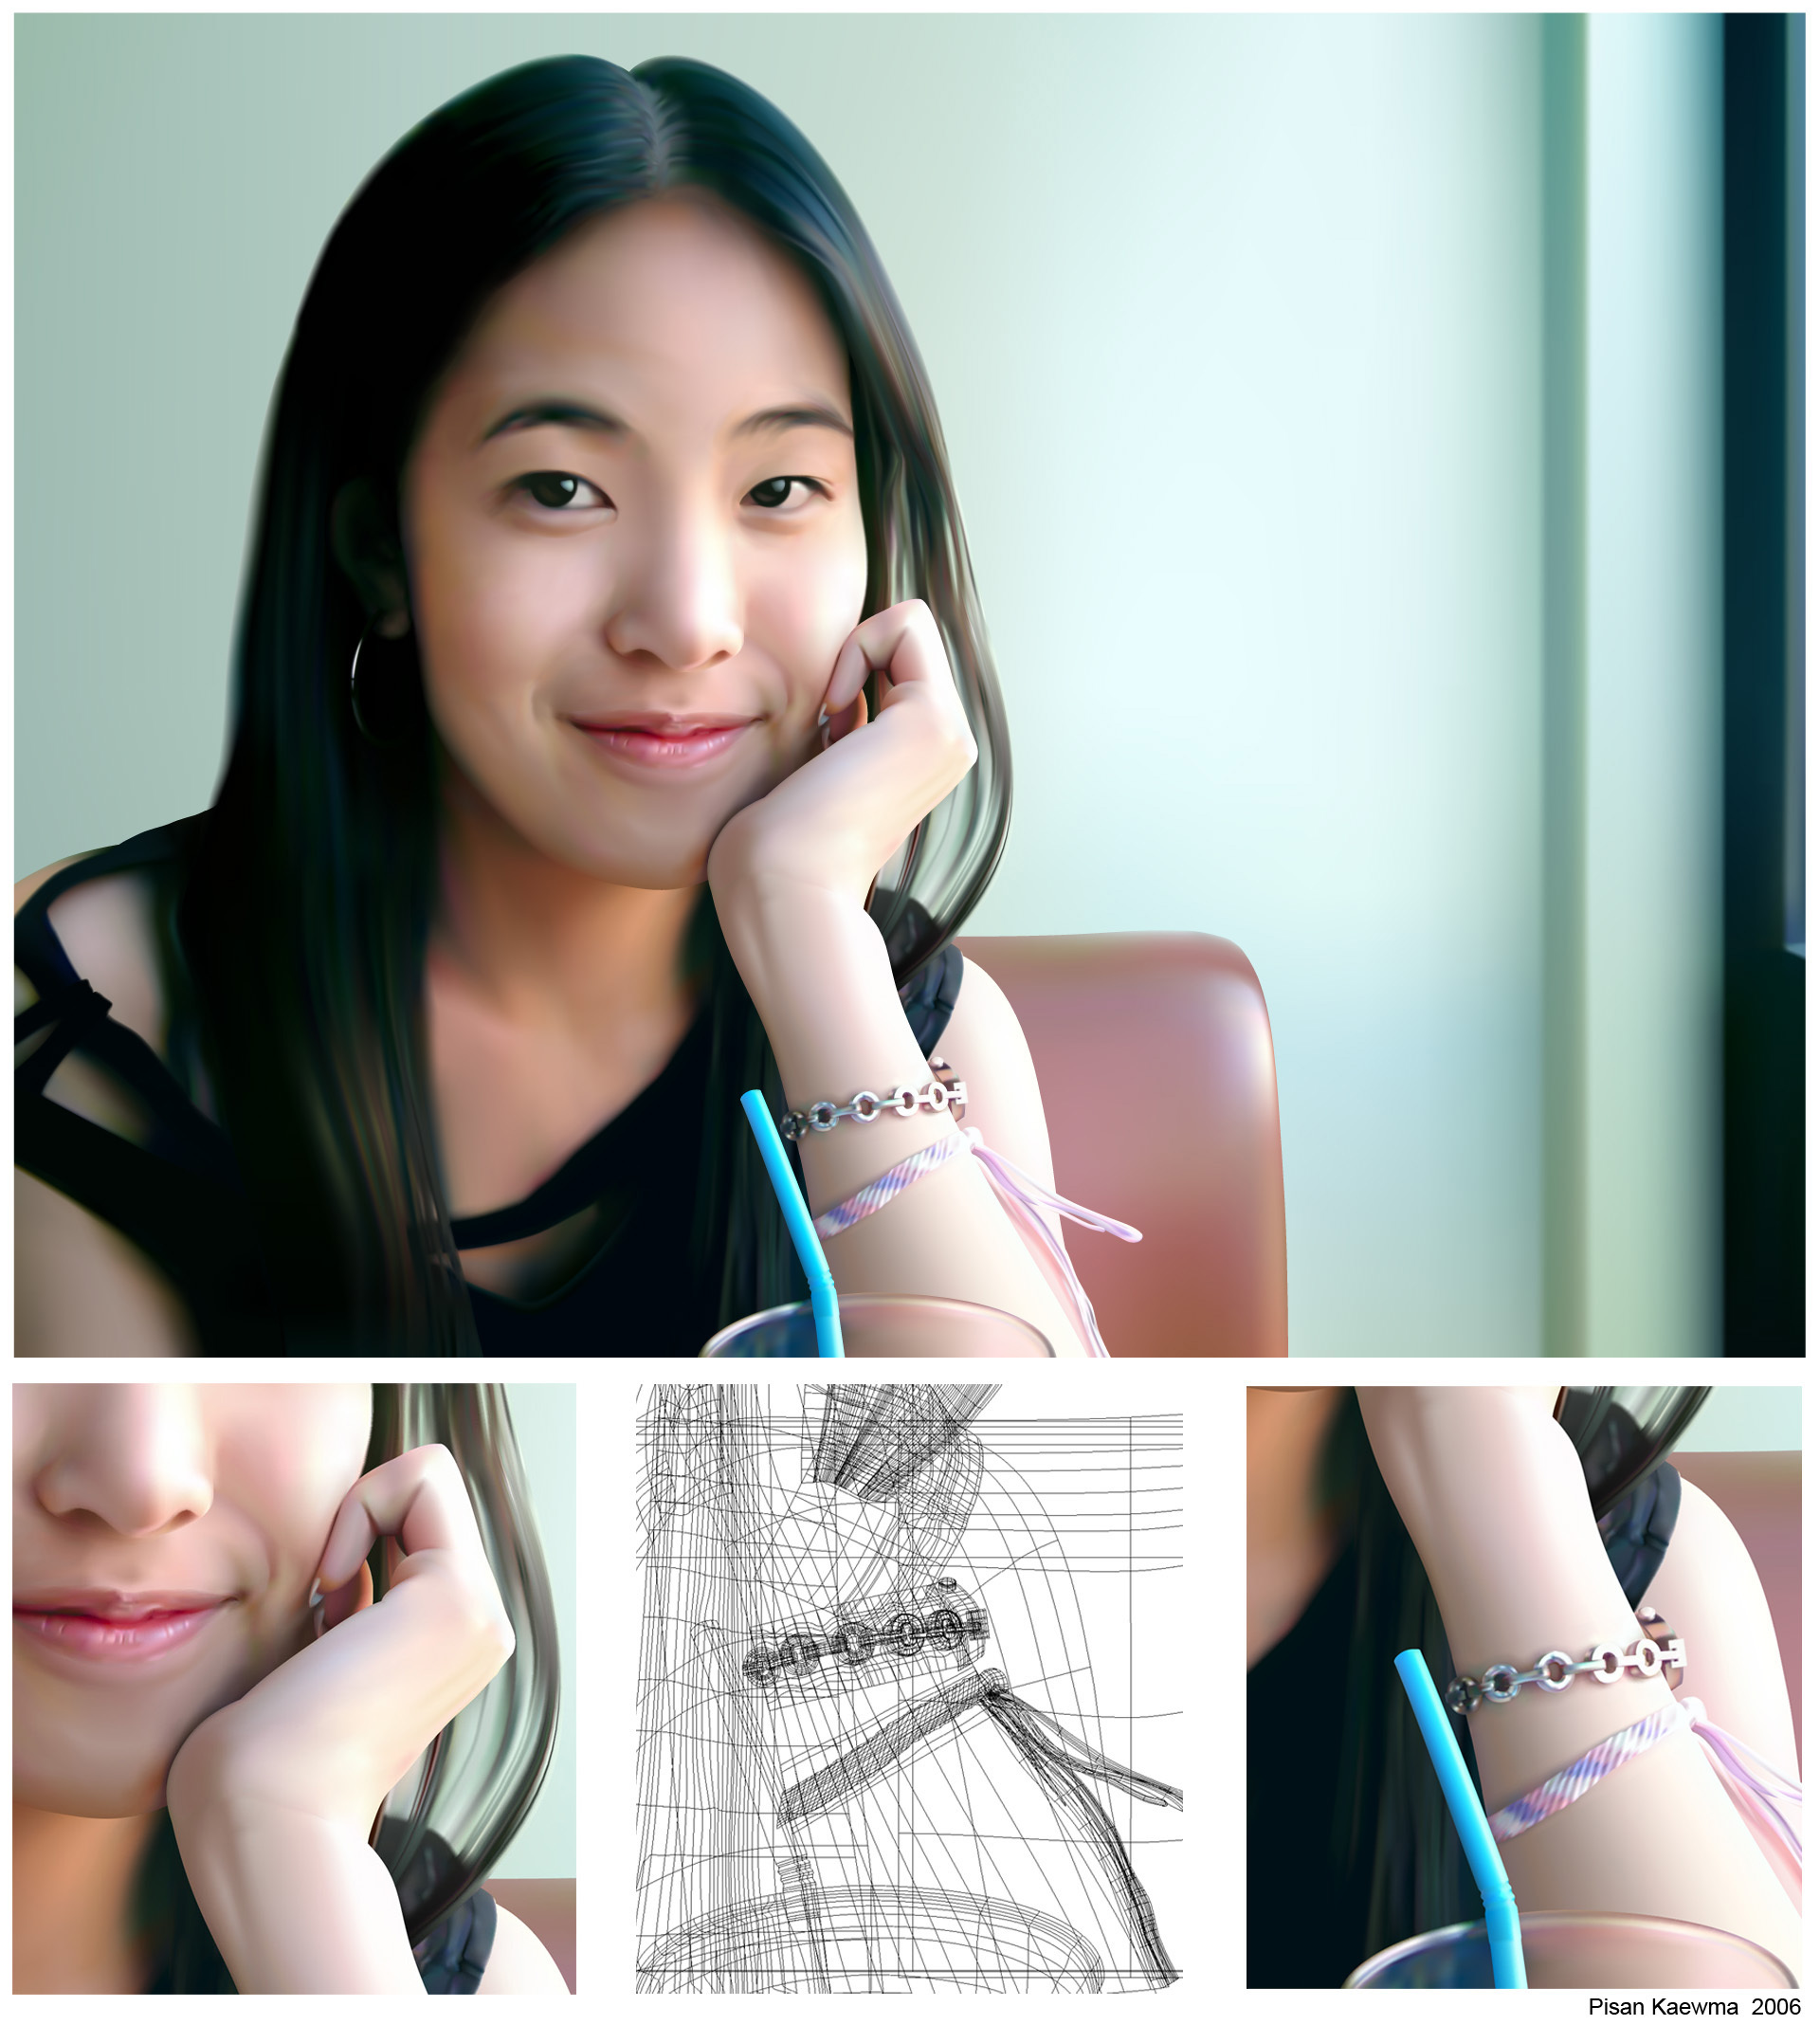
\includegraphics[width=4in]{art/a1336.jpg}
\caption{Ultra realistic vector gradient mesh using Adobe Illustrator by Pisan Kaewma, Thailand}\label{ultra-realistic}
% http://10steps.sg/inspirations/artworks/photo-realistic-vectors/
% http://www.ebypaidrick.com/Gallery.html
% http://www.illustratorworld.com/artwork/1336/
% http://rcpopart.com/labels/hyper-realist%20sculptor.html
% http://www.real-trace.com/index.html
\end{figure}

Recent developments in image processing have made it
possible to find some kinds of artifacts that indicate tampering or wholesale synthesis. For example,
the JPEG compression algorithm produces a mathematical signature when an
image is decompressed, cropped, and then re-compressed. Specular 
reflection, highlights and shadows can be closely examined to reveal
that different objects in a single ``photograph'' actually were
assembled from objects that were in 
slightly different physical environments. In one particular dramatic
demonstration, Dr.\ Hany Farid of Dartmouth University showed that a single ``group picture''
had been created by pasting in the people from different photos
because the reflection of the room lights on each person's eyeballs
were inconsistent with were they were standing in the frame. The technology is now
being commercialized\citep{farid07}.


\subsection{Automated Reasoning}

The leading edge of DF research are systems that
attempt to assist or even automate an analysts' reasoning---systems
that can automatically find evidence that is out of the ordinary,
strange, or inconsistent. Such details can indicate that there is a
deeper, hidden story. Inconsistencies can also indicate that evidence has been
tampered or entirely falsified. 

Ultimately, such automated reasoning systems are likely the only way
that today's analysts will be able to address the vast data
quantities and increasing diversity that they are likely to encounter
in the coming years. There has been some work in this area in
terms of systems that can find timestamp inconsistencies (a file
can't be deleted before it is created), but such rules are invariably
complicated by the messiness of the real world (for example, daylight
savings time). 

\section{The Digital Forensics Challenge}

For all of its power, DF practitioners face stark
challenges in practicing their discipline---challenges likely to
increase in the coming years. Those challenges are size,
time, diversity, cloud computing, encryption and language.

\begin{compactdesc}

\item[Size:] The past three decades have seen a steady increase in the
  amount of storage available to consumers and a steady decline in its
  cost. In 1993 I purchased my first 1 gigabyte external hard drive
  for a thousand dollars; today a 1 terabyte external hard drive can
  be purchased for under a hundred---a thousand times more
  storage for a tenth the price. Not surprisingly, the amount of data
  acquired by law enforcement organizations in their cases is
  increasing every year.

  Alarmingly, other aspects of computing have not scaled as quickly as
  storage. Today's terabyte drives are only 10 to 100 times faster
  than the gigabyte drives of yesteryear, which means that it takes anywhere
  from 10 to 100 times longer to copy  data from the larger
  drives. Likewise, today's computers are only on average 100 fold
  faster than the high-end workstations of the early 1990s, which
  means that there is less computing power available to process each
  byte per unit time. The continuation of these trends means that new techniques are
  required to deal with the data onslaught, as existing techniques
  simply cannot keep up with the increased storage available to consumers.

% My 33Mhz NeXTstation had 10 SPECmarks
% http://www.kevra.org/TheBestOfNext/NeXTProducts/NeXTHardware/NeXTStnColor/files/page620_2.pdf
% Intel Core i7 is 965 SPECmarks
% http://openlab.web.cern.ch/sites/openlab.web.cern.ch/files/technical_documents/CERN_openlab_report-Eval-of-energy-consumption-and-perf-of-Intel's-Nehalem-achitecture.pdf

\item[Time:] Even as the amount of storage received by law enforcement
  organizations increases, the time available to analyze that storage
  is steadily decreasing. In part this is because the number of cases
  in which digital evidence is collected is increasing far faster than
  the number of forensic investigators available to do the
  examinations. But another cause is the increasing realization that
  DF can be used to \emph{solve crimes}---that is, as
  part of the investigation process---whereas in the
  past DF was mainly a tool for \emph{assisting in convictions}. The
  shortened time horizons puts increased demands on tools,
  investigators, and systems.

\item[Diversity:] Forensic investigators must be able to process any
  information found on any computer system currently in use. After
  all, if there were a particular kind of system that could not be
  analyzed, criminals would be sure to use it. Thus, DF tools and
  invesitgators must be able to accommodate all kinds of computers,
  operating systems, application programs and the like. The diversity
  is particularly problematic in the case of cell phones, where there
  are literally dozens of different kinds of cables and tens of
  thousands of apps in widespread use that might require analysis.

\item[Cloud Computing:] Further complicating the investigator's job is
  the emergence of cloud computing and other technologies for storing
  data in the Internet rather than on desktops, laptops, and mobile
  devices. As a result of the cloud, there is no way to assure that a
  seized cell phone actually holds the suspect's data---the phone
  might simply be a tool for accessing a remote server. A law
  enforcement professional who is authorized to search a device may
  not have legal authority to use information on that device to access
  remotely stored data. Worse still, the data might be deleted in the
  meantime by one of the suspect's collaborators.

\item[Encryption:] The increased use of encryption means that
  investigators might not be able to decipher information once they
  have it in their possession. 

\item[Language:] Finally, in today's global environment forensics
  examiners are increasingly encountering evidence written in human
  languages that the examiner does not understand. And while tools
  like Systrans and Google Language Tools can perform some automated
  language translation, such systems are rarely sufficient for
  real-world forensic media.

\end{compactdesc}

These challenges impact the entire forensic processing model. Here are
two  examples:

\begin{compactitem}
\item Ten years ago it was relatively easy to collect and preserve a
computerized evidence: standard procedure was for law enforcement to
turn off a suspect's computer and take it back to the police station
where it might be put in an evidence locker. But modern computer systems
frequently employ encryption: turning them off may cause a key to be
erased, eliminating the possibility of decrypting the data without the
suspect's cooperation. For these systems it is now common practice to
copy out the computer's memory if possible---except that it is not
always possible because of diversity. 

\item Cell phones may be equipped with ``self destruct'' applications
  that wipe their data if they receive a particular text, so it is now
  standard practice to store phones in a shielded metal box called a
  Faraday cage that blocks radio waves. But many cell phones forget
  their storage if left off for too long, so the Faraday cages must be
  equipped with power strips and cell phone chargers.  Because many
  low-end cell phones have proprietary plugs, police must seize chargers as well.
\end{compactitem}


\subsection{The Research Agenda}

  Addressing these increases has only been possible through the
  collective research of government agencies, academics, and
  independent practitioners. These research efforts largely fall into
  three areas:

\begin{description}
\item[Reverse Engineering] has traditionally been the most basic form
  of DF research. Developers generally do not provide the public
  with details of how their systems work. This is obviously true of
  malware developers, but it is also true of legitimate companies that
  develop hardware and software, and even many open source
  systems. As a result, forensic practitioners must expend
  considerable effort reverse engineering systems to  understand how
  they work.  Today's techniques to extract allocated files from disk
  images were largely developed through reverse engineering.

\item[System Analysis] is the second leg of forensic research. System
  analysis is the systematic exploration of digital systems to
  understand the information that they contain and how it can be
  exploited for forensic analysis. Although similar to reverse
  engineering, system analysis is fundamentally different, in that the
  information the system analyst seeks may be unknown to the
  developers themselves. Although this may seem strange, remember that
  computers are vastly complicated systems: just as programmers
  frequently put bugs in their programs without realizing it, programs
  invariably have other behaviors that aren't bugs but are equally
  unforeseen by the original programmers. Many system users and quite
  a few developers assumed that it was not possible to recover deleted
  files until data recovery experts developed tools that proved otherwise.

 As long as there is data data that exists but which cannot be viewed
 through the operating system, there is need for tools that can
 display it. There is simply no commercial reason for software vendors
 to create tools which make this information visible---in many cases
 they are not even aware that the data is present. For example,
 previous versions of Microsoft Word left text in a
 document file even after it was deleted because the software didn't
 explicitly wipe the memory and corresponding disk sectors that
 corresponded to each deletion. This deleted-but-recoverable text
 occasionally resulted in some embarrassing revelations---so much, in
 fact, that many Microsoft products now explicitly have commands for
 to ``remove hidden data.'' Computer forensics tools can be
 used to both demonstrate the problem and verify whether or not
 Microsoft's solution actually works.

\item[Advances in fundamental science and engineering] are also needed
  for advances in DF. In particular, today's DF researchers are at the
  forefront of many other hot fields in computer science, including
  cloud computing, big data, visualization, and natural language
  processing. File carving and the recovery of data from corrupted
  compressed files are both examples of this kind of work: much of
  this work was thought to be computationally prohibitive until new
  mathematical algorithms were developed that proved
  otherwise. Another example is software that automatically translates
  posts on Facebook and Twitter from the subject's native tongue into
  a human language that the examiner can understand.
\end{description}


\subsection{The Biggest Challenge: Human Capital}

Despite its technical sophistication and reliance on the minutiae of
digital systems, the single biggest challenge facing digital forensics
practice today has a decidedly human dimension: the lack of qualified
people to serve as DF researchers and practitioners. But the human
resources problem faced in forensics is not merely the result of the
general tech shortage: the very nature of digital forensics makes our
human resources problem significantly harder than faced by other
disciplines. 

Because DF's mission is
to understand any data that might be stored on a computer
system, we need individuals that have knowledge
of both current and past computer systems, applications, and data
formats. We need generalists in a technological society that
increasingly rewards experts and specialization. 

This human resource problem is a bigger barrier to the
future of forensics than 
any technological problem that we have ever encountered. Whereas full
disk encryption might prevent a single hard drive from being
deciphered, the lack of skilled individuals can lead to backlogs of
months or longer---preventing evidence from even being collected.

One way to address this training problem is to look for opportunities
to modularize forensic problems so that experts in related fields can
make meaningful contributions. 

I believe that another approach is to show how the underlying
principles and current tools of digital forensics can be widely
applied throughout our society. This will increase the research of DF
tools and hopefully, as a result, increase the user base of the software.

For example, many of the tools of digital forensics can be used
for privacy auditing. That is, instead of using the tools to find
personal information that might be relevant to a case, businesses and
individuals can use the tools to look for the inappropriate presence of personal
information left behind because of bugs or oversight. (I am currently
writing a textbook on this topic.) Likewise, individuals can use tools
like file carvers to recover photographs that have been accidentally
deleted from digital cameras.

More generally, as our cars, street signs, communication systems,
electrical networks, building materials, and even companions are
increasingly computerized, digital forensics is likely to be one of
the only way for understanding these systems when they misbehave---or
when they are subverted. The increased computerization of our society
assures the continuing need for forensics capabilities and
practitioners. But without fundamentally new approaches for developing
these tools and capabilities, the difficulty and cost of forensic analysis is likely
to increase along with the ever-expanding data sizes and system
complexity. It's not just an arms race between investigators and the
criminals that they are hunting, but between the investigators and the
developers of tomorrow's computer systems.

\section{Terminology}
\begin{description}
\item[Allocated (files and sectors)] Allocated files are files that can be viewed through
  the operating system; allocated blocks are blocks that have been
  allocated to a specific file and will not be re-used by the
  operating system unless the contents are first relocated
  elsewhere. cf with \emph{deleted files}.
\item[Bit] A binary digit (0 or 1). The word ``bit'' was coined by
  John W.\ Turkey (1915-2000) while working at Bell Labs and first appeared in
  print in Claude Shannon's seminal 1948 article on information
  theory, \emph{A Mathematical Theory of Communication}. (Turkey also
  coined the word \emph{software}.) Abbreviated with a lower-case
  letter \emph{b}.
\item[Byte] An ordered set of bits used to represent the minimum
  amount of data that can be read or written to a computer memory at a
  time. Modern computers use 8-bit bytes, allowing for 256
  ($2^8$)possible values (typically 0 through 255 if the byte is
  interpreted as an unsigned number, or -128 through 127 if the byte
  is interpreted as a signed value.) Abbreviated with an upper-case
  letter \emph{B}.
\item[Compression] A mathematical process for reducing the size of a
  file or other digital object. Compression can be \emph{lossless} or
  \emph{lossy}. In Lossless compression the original file can be recovered by
  \emph{decompressing}, while with lossy compression information is
  lost and the exact original cannot be recovered. (However, lossless
  compression may have such high fidelity that a human being is unable
  to distinguish between the original and the decompressed objects.
\item[Deleted files] Files whose contents can be recovered but the
  sectors of which are not allocated.
\item[Digital Forensics] ``A branch of forensic science encompassing the
  recovery of and investigation of material
  found in digital devices, often in relation to computer crime.''\cite{reith:examination}
\item[Digital Trace Evidence] Another name for \emph{residual data}.
\item[Disk Image] A byte-for-byte copy of all the data on hard drive,
  camera card, or other kind of sector-oriented mass storage
  device. Disk images can contain additional metadata such as an
  embedded cryptographic hash of the original media, the date that the
  image was made, the examiner who made the image, as well as notes.
\item[Disk Imager] A program for making disk images.
\item[Media Exploitation] The extraction, translation and
  analysis of digital documents and media to generate
  useful and timely information.
\item[File] An ordered collection of 0 or more bytes. Files have a
  length; they may optionally metadata such one or more file names,
  modification dates, owners, and other information.
\item[File Header] One or more fixed bytes at the beginning of a
  file. For example, ZIP files begin with the file header ``PK'' (hex
  \texttt{50 4B}), while JPEG files begin with the field header
  \texttt{FF D8 FF E0}.
\item[File Footer] One or more fixed bytes at the end of a file. JPEG
  files end with the file footer \texttt{FF D9}.
\item[File System] Part of a computer's operating system which
  controls the storage of files on a mass storage system such as a
  hard drive or camera card.
\item[Forensic Science]
\item[Hash Value] Always say \emph{hash value}, never \emph{hash
  code}, since the word \emph{code} might refer to either the hash
  value or the program that computes the value.
\item[Investigator-Centric] Digital Forensics is said to be
  ``investigator-centric,'' meaning that most of the advances in the
  field have been to serve specific needs of investigators, rather
  than based on what is scientifically or technically possible.
\item[Logical Block Address (LBA)] \emph{Sectors} of a mass storage
  device are arranged in numbered sectors, starting with LBA 0. Early
  PC systems used hard drives that supported a 22-bit LBA and 512-byte sectors, allowing for a
  total of $2^{22}\times 2^{9}=2^{31}=2\textrm{TB}$ of storage. The
  current Advanced Technology Attachment standard, ATA-6, supports
  48-bit LBA addresses and a 4096-bit sector size, for a maximum disk
  with $2^{48}\times 2^{12}=2^{60}\approx 1,152,921\textrm{TB} \approx 1
  \textrm{EB (exabyte)}$ of storage.
\item[Malware] Software that embodies evil intent, such as to damage
  computer systems or steal private information. Computer Viruses,
  worms, and Trojan horses are examples of malware. 
\item[Metadata] Data about other data. The created, modified and
  access timestamps associated with a file on a camera card are
  examples of metadata.
\item[MD5] Message Digest \#5, a cryptographic hash algorithm
  developed by MIT professor Ron Rivest in 1991. Although MD5 is
  widely used in computer forensics, MD5 has known flaws and should
  not be used in applications that depend upon collision resistance.
% \item[Network forensic analysis tool (NFAT)] A system that can record
%   packets as they move over a network and perform detailed
%  after-the-fact analysis.
% \item[normalization]
% \item[Packet] A set of bytes that are sent over a network. Most
%   Internet packets range in size from 40--1500 bytes.
% \item[PCAP File] A packet capture file, which is typically a set of
%   packets that were recorded using a packet sniffer.
% \item[Packet sniffer] A program or device that can record packets are
%   they move over a network.
% \item[Packet Traces]
% \item[Provenance]
\item[Residual Data] data that is left behind on a computer after an
  operation is completed but is no longer in active use. For example,
  most computer systems erase the file name when a file is deleted,
  but do not overwrite the actual file contents. These contents remain
  on the drive as residual data, recoverable with computer forensic tools.
\item[Sector] The minimum amount of data that can be read or written
  to a mass storage device. Modern hard drives use sectors of 4096
  bytes; drives with 512-byte sectors have been common since the mid
  1970s and are still widely used today.
\item[Subject Computer and Data] The computer system and data that are
  being analyzed as part of a digital investigation. This may be data
  extracted from a computer belonging to a suspect in a crime, but it
  may also be data from the computer of a victim. Subject data may
  even be data generated during the course of a DF tool.
\item[Subject] is a common shorthand for the owner or primary use of a computer
  system from which subject data was obtained. 
\item[Tool-Based] Digital Forensics is said to be ``tool-based,''
  meaning that most investigators in their investigations to the
  capabilities provided by today's tools---investigators generally do
  not devise their own digital experiments or invent new approaches
  for working with data to solve specific cases.
\item[Timestamp]
\item[Unallocated sectors] Sectors that are not allocated to files or
  metadata, but are instead available for use by the file system
\end{description}


% LocalWords:  probative centric transformative Merkle combinatorial modularize
% LocalWords:  Ponzi Specular DF Madoff pre GPS Cyber imager
      1
%\chapter{Forensic Containers and Forensic Device Imaging}
The introduction of digital forensics into law enforcement as a formal
practice in the 1990s made two differences between traditional
forensics and digital forensics abundantly clear:
\begin{compactenum}
\item Whereas a major challenge with traditional forensics is the
  securing of the crime scene and the collection of representative
  evidence, it is relatively straight-forward to isolate a ``digital
  crime scene'' by turning off a computer and removing its hard
  drive. 
\item Whereas in the physical world it is generally possible to
  prevent or at least detect inadvertent (or intentional) damage to
  evidence, it is generally possible to make undetectable
  changes to digital evidence.  For example, it can be generally determined through
  forensic examination that a page has been torn out of a notebook,
  but it is generally not possible to tell that a sector that
  containing an email  address such as \emph{user1234@aol.com} was
  overwritten to read \emph{usr3@hotmail.com}.
\end{compactenum}

The original purpose of \emph{forensic containers} was to overcome
both of these limitations by providing a facility for making a copy of
data that was faithful to the original and for which 
subsequent changes to the contained data could be detected. Since then
a number of other requirements have emerged, as shown in
\tabref{container:requirements}. The Advanced Forensic Format version
3\cite{garfinkel:aff} is the only forensic container format that
currently satisfies all of these requirements.

In addition to those requirements, it
can be useful for evidence containers to provide additional
functionality, including:

\begin{table}
\begin{itemize}
\item Provide a general purpose facility for  storing case information.
\item Provide an integrity check on the contents of the evidence. This
  is typically implemented with a cryptographic hash.
\item Provide a digital signature on the evidence, typically provided
  by signing the cryptographic hash with a private key. Ideally this
  signature should be created with a key that is embedded in the
  device that acquires the evidence using a hardware security module.
\item Likewise, evidence containers should provide for integrity
  checks and digital signatures for metadata.
\item Allow evidence and metadata to be encrypted so that it cannot be accessed
  by unauthorized parties. Encryption can be performed using a
  password, a symmetric encryption key, or an asymmetric key. The use
  of an asymmetric key (for example, an X.509 public key certificate)
  allows evidence to be acquired in the field in such a way that it
  cannot be reviewed by those who acquire it, and can only be decoded
  when the evidence is returned to the lab where the private key
  resides.
\item Maintain a record of the evidence provenance, including the device from which the evidence was
  extracted, who did the extraction, what tools were used, when and
  where the extraction took place, and other similar information.
\item Maintain a record of the evidence chain-of-custody as it moves
  from one data custodian to another.
\end{itemize}
\caption{Requirements for a digital evidence container.}\label{container:requirements}
\end{table}


\begin{itemize}
\item Provide for the exchange of evidence and forensic
  work product between different examiners and different tools.
\item Store intermediate results, reducing the need for
  reprocessing evidence and speeding the examination process.
  Typical intermediate results include cryptographic hashes of files
  and full-text indexes of file contents.
\end{itemize}

Most forensic containers in use today provide integrity checks for
evidence but not for metadata. TK

\section{Background}

This chapter is primarily concerned  with the collection and preservation of
digital information from \emph{mass storage} or \emph{secondary
  storage} devices. 

\emph{Storage} is a term that is used in computing to refer to a
system that can hold information and allow the information to be
retrieved at a later point in time. 

In computing the word \emph{store}
is used both as a verb (the act of storing the information) and a noun
(the place where the information is stored). Computer systems have two
kinds of storage systems:

\begin{description}
\item[Primary Storage] is storage that can be directly accessed by the
  computer's central processing unit (CPU). Most computers use
  \emph{Random Access Memory} (RAM) as their primary storage, although
  some systems can also use a special kind of flash memory called
  \emph{NOR Flash}. 

\item[Secondary Storage] is storage that cannot be directly accessed
  by the CPU. To use secondary storage, information must be copied
  between secondary storage and primary storage. Typically these copy
  operations are performed on fixed-sized \emph{blocks} of data.
\end{description}

Even though this chapter is concerned with data on mass
storage system, we will see that forensic containers need to be able
to store a wide variety of other kinds of information, including
network packets, memory dumps, and even individual files. These
additional modalities are required for a variety of reasons:

\begin{itemize}
\item Data from networks or memory is frequently found on subject hard
  drives. When it is found, it is useful for the forensic examiner to
  extract that data and store it in its own container. 
\end{itemize}

\subsection{Storing Bits, Bytes and Sectors with Mass Storage Systems}

Computers store information in digital form, that is, as a series of
0s and 1s called \emph{bits} (short for ``binary digit'').

Modern computers do not work with bits directly, but use sequences of
8 bits called bytes. This sequence can represent
$2\times2\times2\times2\times2\times2\times2\times2=2^8=256$ distinct
values. The meaning assigned to these values generally depends on the
context. A few examples are shown in \tabref{tab:8bits}. The ASCII
codes represent NULL (no data is sent), SOH (Start Of Heading---the
beginning of a data header), and DEL (delete). NULL is a holdover from
the days of synchronous terminals, when there needed to be a constant
flow of data down all links: sending all 0s (NUL) meant that the data
should be ignored. DEL was chosen as delete when characters were
punched on paper tape and cards: in the event of an error, the
operator could backspace the punch and punch holes across the entire
line, causing the computer to ignore the value. We shall return
to the question of representation in \chapref{chap:unicode}.

\begin{table}
\begin{tabular}{cccccccc|c|c|c|c}
\multicolumn{8}{r}{                       Term:}  & unsigned char & signed char & ASCII \\
\multicolumn{8}{r}{                       Range:} & 0--255      & -128--127 & NULL--DEL\\
\cline{9-11}\multicolumn{8}{c}{Bits}                          &        &               &             &          \\
$2^7$ & $2^6$ & $2^5$ & $2^4$ & $2^3$ & $2^2$ & $2^1$ & $2^0$  &        &               &             &          \\
  128 &    64 &   32 &    16 &     8 &     4 &     2 &     1  &        &               &             &          \\
\hline
    0 &     0 &    0 &     0 &     0 &     0 &     0 &     0 &            0  &            0  &   NULL     \\
    0 &     0 &    0 &     0 &     0 &     0 &     0 &     1 &            1  &            1  &   SOH      \\
    0 &     1 &    0 &     0 &     0 &     0 &     0 &     1 &           65  &           65  &   A        \\
    0 &     1 &    1 &     0 &     0 &     0 &     0 &     1 &           96  &           65  &   a        \\
    0 &     1 &    1 &     1 &     1 &     1 &     1 &     1 &           127 &          127  &   DEL      \\
    1 &     0 &    0 &     0 &     0 &     0 &     0 &     0 &           128 &         -128  &   n/a      \\
    1 &     1 &    1 &     1 &     1 &     1 &     1 &     1 &           255 &           -1  &   n/a      \\
\end{tabular}
\caption{Eight bits can represent 256 distinct values.}\label{tab:8bits}
\end{table}

As indicated above, while the primary storage system of most computers can be accessed a
byte at a time, secondary storage can only be accessed in
blocks. Secondary storage, in turn, can be divided into two broad
categories:

\begin{description}
\item[Block addressable] storage systems are systems for which any
  block can be individually read or written. Each block in a block
  addressable system is assigned a \emph{logical block address}
  (LBA). 
\item[Streaming] storage systems are those that allow blocks to be
  read or written as part of a sequence. Most streaming systems are
  based on a spool of magnetic or optical tape. New blocks can be
  written to the tape and the tape supports limited operations---for
  example, \emph{rewind}, writing a \emph{mark}, \emph{seeking} to a mark,
   \emph{erasing} and possibly \emph{overwriting}. In general it is
   not possible with a streaming system to reliably overwrite a single
   block---attempts to do so may result in other blocks being damaged
   and rendered unreadable.
\end{description}

Confusingly, although we have used the term \emph{block} exclusively
until now, many vendors use the term \emph{sector} to describe blocks
that are written to spinning discs. (The term is presumably comes from
the fact that data was originally stored in concentric circles on a spinning platter
and in bands on a rotating magnetic drum. Thus, each block occupied a
sector of a circle.) Until the mid 2000s most mass storage systems
used blocks (sectors) that were 512 bytes in size. Since then vendors
have moved to systems that use 4096-byte blocks internally, although
many still give the appearance of using 512-byte sectors to provide
for software compatibility. 

\subsection{How many bytes? GB vs. GiB}

There are two standards used in computing to represent the size of a
storage system: SI (the International System of Units) decimal
prefixes and IEC (International Electrotechnical Comission) 60027
binary prefixes. This situation is confusing because until recently
the SI prefix names \emph{kilo}, \emph{mega} and \emph{giga} were used
both to decimal and binary notation, the correct multiplier being
inferred from usage. Today there is an effort underway to clarify
usage. This section describes correct usage and provides hints for
determining when usage is incorrect.

SI decimal prefixes are commonly used to represent metric
quantities. The SI prefix ``giga'' multiplies the following value by $10^9$; thus a gigabyte (GB) is
$10^9=1,000,000,000$ bytes. Confusingly, this is called a ``billion
bytes'' in the US but a ``thousand million'' bytes in Great Britain.

The IEC 60027 prefix ``gibi'' multiples the following value by $2^{30}$. A gibibyte
(GiB) is thus $2^{30}=1,073,741,824$ bytes. At least, this has been
proper usage since 1999 when the IEC adopted 60027-2 for binary
prefixes. 

The confusion dates back to the early 1990s. At the time the SI
prefixes were widely used in the computing industry to as binary
multiplier: \emph{kilobyte} meant 1024 bytes, \emph{megabyte} meant
$1024\times1024=1,048,576$ bytes and a \emph{gigabyte} (an
unimaginable amount of memory at the time) meant
$1024\times1024\times1024=1,073,741,824$ bytes. These terms were most
commonly used to describe the size of primary memory systems. Because
the systems were addressed with binary address lines, a system with 24
address lines could address $2^{24}=16,777,216$ bytes of
memory. Terminology at the time was to say that such a system had a
``sixteen megabyte address space.''

Vendors of mass storage systems had long realized that they could
save money by rating their storage systems using the true meaning of
the SI prefixes. That is, a hard drive sold as being a ``100 gigabyte
hard drive'' could legitimately be sold with 100,000,000,000 bytes of
physical storage. Assuming 512-byte sectors, such a system would only
need to have:
\begin{equation}
\frac{100 \times 10^9 \textrm{~bytes}}{512 \textrm{~bytes per sector}}=195,312,500 \textrm{~physical sectors}
\end{equation}

However, if the hard drive vendor adopted common usage at the time, a
``100 gigabyte'' drive would actually need to have:
\begin{equation}
\frac{100 \times 2^{30} \textrm{~bytes}}{512 \textrm{~bytes per sector}}=209,715,200 \textrm{~physical sectors}
\end{equation}
Unlike primary storage, secondary storage is addressed by sending a
logical block address down a bus. There is no technical advantage to
filling out the last 10 million sectors, and for hard drive vendors
there is a real cost to insuring that an additional 10 million usable
sectors are present on the drive. 

None of this was a problem as long as purchases were confined to a
relatively small group of informed individuals. But as the market for
storage systems increased, so did the confusion. As a result, the IEEE
Standards Board realized that it could not change the SI prefixes for
computing, and instead adopted a new set of prefixes to describe
binary multipliers. (See
\url{http://physics.nist.gov/cuu/Units/binary.html} for more information.)

\subsection{Drives, Hard Drives, Solid State Drives}

\subsection{Write Blockers}

Removable media such as floppy disks, tapes and storage cartridges
used in the 1990s generally had some kind of \emph{write-protect}
switch or tab that could be used to prevent inadvertant alternation or
overwriting of evidence. Hard drives of the time had no such
facility. To overcome this deficiency the industry invented
\emph{write-blockers}, a device that can be inserted inline between a
hard drive and a computer system. A typical write blocker might have a
male and a female ATA-33 connector; the female connector plugs into
the hard drive's male ATA-33 connector, while the blocker's male
connector plugs into a cable that connects to the host computer.

Write blockers allow examination of subject data without fear of
inadvertently modifying the contents---provided that the write blocker
works properly. A problem with the concept of write blockers is that
the only real specification of what these devices should do was their
name---that is, they should block modification of data on the hard
drive.  But there
are two ways to do this. One is to literally block the commands that
alter data, a task that requires a clear enumeration of all such
commands. An alternative (and somewhat safer) strategy is to only pass
those commands that are known \emph{not} to alter
data\cite{dfrws2006:JamesLyle}. Both of these approaches
implicitly assume that the only way data is altered on the drive is
through the execution of commands, and this is not actually the
case. For example, the S.M.A.R.T. counters inside modern drives that
track the number of seconds the drive is powered up will continue to
advance even when a write-blocker is in place.

\subsection{Disk Imaging and Disk Images}
Two problems that are not solved by write blockers. First, the
digital evidence still resides on the original media, which is a
mechanical device and subject to failure. Second, most legal systems
allow for both parties to have access to evidence. Both of these
problems can be overcome by making a sector-for-sector copy of the
disk, a process called \emph{disk imaging}.

The most basic way to image a disk is to copy every sector onto
another disk of the manufacturer and model number. Such a disk is
called a \emph{mirror copy} or \emph{mirror volume}. Once the copy is made, the subject disk
can be kept sealed in an evidence locker and the mirror volume can be
used for forensic analysis. 

A difficulty in making a mirror copy is that it may not be possible to
obtain a drive of the exact make and model number. Fortunately, it is
only necessary for the copy disk to be larger than the original. The
sectors between the end of the original disk and the copy disk should
be ignored.

[Figure: original disk, copy, and the section to ignore.]

\citeN{dfrws2002:JamesLyle} introduced the Computer Forensic Tool Testing (CFTT)
program at the National Institute of Standards and Technology (NIST).

\subsection{Inaccessible Information}

TK - DCO and HPA

TK - SMART information

\section{Image Files}
Instead of making a copy to a mirror disk, it is possible to copy all
of the accessible blocks on a mass storage system into a single file
on a computer disk. Such files are called \emph{image files} because
they represent an image of the information stored on the disk. The
term ``image'' here should not be confused with the other usage of the
word ``image'' to describe a photograph.

A raw disk image is a byte-for-byte copy of a mass storage
system. Such files can be quite large---a 256GB drive will have a raw
image that is 256GB in size. This can cause problems, as many computer
systems cannot operate on files that are larger than 2GiB or 4GiB due
to 32-bit limitations. One way to address the file size limitation is
by splitting the file into multiple files of equal size---for example,
a 256GB disk image can be split into 256 files of 1GB each. Such
collections of files are called \emph{split raw images}; each file is
typically given a name such as \emph{FILENAME.000}, \emph{FILENAME.001},
\emph{FILENAME.002} and so on.

A second and more important problem with raw image files is that they
lack important \emph{metadata} about the process by which they were
acquired. Metadata is data about data; in the case of files in a file
system the metadata includes the file's name, timestamps, and other
kinds of file system information. But in the case of disk images,
there is a wealth of additional metadata that can be collected, such
as:

\begin{itemize}
\item The date and time that the disk was imaged.
\item The manufacturer, model number, and serial number of the disk
  that was imaged.
\item The examiner that did the imaging.
\item The physical location where the image was made.
\item Other notes about the imaging process or the physical artifact.
\end{itemize}

There is also need for integrity controls to assure that the disk was
properly imaged and that the image itself was not altered or corrupted
after the file was created. A common integrity control is to compute
the cryptograhpic hash of the disk image's bitstream, computed by
feeding all of the bytes in the disk image into a hash function such
as MD5 or SHA1. Cryptographic hashes have the property that changing a
single bit causes the resulting hash function to change
unpredictably. In practice, the examiner computes the hash of the disk
image and stores this information separately---for example, by writing
it in a notebook. The disk can then be imaged a second time. If the
two disk images have the same hash, then the examiner can assume that
the image itself is a faithful copy of the source disk. Later, the
examiner can re-calculate the hash of the disk image to show that the
image has not been modified.

Compression can significantly shrink the size of a disk image
file. Although it is tempting to such programs such as ZIP and GZIP
directly on a raw file, the resulting file must be entirely
decompressed before it can be used. For files larger than a gigabyte
this quickly proves unworkable. Instead, it is common practice to
use a file format that breaks the raw disk image into blocks or
segments and compresses each individually. These segments are then
stored in the resulting image file, along with some kind of map that
describes, for each segment, the offset within the original uncompressed file
and the physical offset of the compressed segment in the compressed file.

[Diagram showing the original file, the compressed file, and the map]

\subsection{Image File Formats}
Today a wide number of image file formats are in use. Broadly
speaking, there are formats that were developed for digital forensics
and those developed for mainstream computing. Within the set of
formats developed for digital forensics, there are \emph{proprietary formats} that were developed by
vendors for commercial tools and \emph{open source} formats that were
largely developed for academic purposes. However the distinction can
be misleading, as there exists several open source implementations for
the proprietary formats, making them somewhat open source. 

\subsubsection{Proprietary Forensic Formats}

SafeBack~\cite{safeback}, a DOS-based utility designed to create
exact copies of entire disks or partitions, offers a
``self-authenticating'' format for images, whereby SHA256 hashes are
stored along with data to ensure the latter's integrity.  Although
few technical details are disclosed publicly, SafeBack's authors
claim that the software ``safeguards the internally stored SHA256
values''~\cite{safebacksafeguards}.


The most widely disk image format appears to be Guidance Software's EnCase Forensic~\cite{encase} uses
a proprietary format for images, reportedly based on ASR Data's
Expert Witness Compression Format~\cite{ew}.  EnCase's Evidence File
(.E01) format~(Fig.~\ref{fig:encase}) contains a physical bitstream
of an acquired disk, prefixed with a ``Case Info'' header,
interlaced with CRCs for every block of 64 sectors~(32 KB), and
followed by a footer containing an MD5 hash for the entire
bitstream.  Contained in the header are the date and time of
acquisition, an examiner's name, notes on the acquisition, and an
optional password; the header concludes with its own CRC. 

The E01 format allows for the contents of a disk image to be
compressed. Each image volume contains a so-called ``jump table'' that
contains the offset of each block in the original uncompressed disk,
the offset in the disk image of the compressed block, and the size of
the compressed block. Originally offsets were described with 32-bit
signed integers, limiting the size of the disk image volume to 2GiB;
additional volume files with extensions E02, E03, and so on could be
added to create images of disks that could not fit within a single
volume. The EnCase imager allows the user to specify a maximum size
for each of these files: setting the size to 700MB allows each volume
to be burned to a CD-R. 

AccessData's Forensic Toolkit (FTK)
supports storage of disk images in EnCase's or SMART's file format,
as well as in raw format and an older version of Safeback's format
(Section~\ref{sec:safeback}). 

\subsection{ILook Investigator's IDIF, IRBF, and IEIF Formats}
ILook Investigator v8~\cite{ILookv8} and its disk-imaging
counterpart, IXimager, offer three proprietary, authenticated image
formats: compressed (IDIF), non-compressed (IRBF), and encrypted
(IEIF). Although few technical details are disclosed publicly,
IXimager's online documentation~\cite{IXimager} provides some
insights:  IDIF ``includes protective mechanisms to detect changes
from the source image entity to the output form'' and supports
``logging of user actions within the confines of that event;''  IRBF
is similar to IDIF except that disk images are left uncompressed;
IEIF, meanwhile, encrypts said images.

For compatibility with ILook Investigator v7 and other forensic
tools, IXimager allows for the transformation of each of these
formats into raw format.

\subsection{ProDiscover Family's ProDiscover Image File Format}
Used by Technology Pathways' ProDiscover Family of security tools
\cite{prodiscover}, the ProDiscover Image File format
\cite{prodiscoverformat} consists of five parts: a 16-byte Image
File Header, which includes a signature and version number for an
image; a 681-byte Image Data Header, which contains user-provided
metadata about the image; Image Data, which comprises a single block
of uncompressed data or an array of blocks of compressed data; an
Array of Compressed Blocks sizes (if the Image Data is, in fact,
compressed); and I/O Log Errors describing any problems during the
image's acquisition.

Though well documented, the format is not extensible.


\subsubsection{Open Source Forensic Formats}

Supported by PyFlag\footnote{In addition to its own {\tt sgzip} format,
PyFlag can also read and write the Expert Witness Compression Format
\cite{pyflagiosources}.}~\cite{pyflag}, a ``Forensic and Log
Analysis GUI'' begun as a project in the Australian Department of
Defence, {\tt sgzip} is a seekable variant of the {\tt gzip} format.  By
compressing blocks (of 32KB, by default) individually, {\tt sgzip} allows
for rapid accessing of the disk image by forensic software without the
need to first decompress the entire image. The format does not associate metadata with images.
\cite{pyflagdiskforensics,pyflagiosources}



\citeN{dfrws2005:PhilipTurner} introduced \emph{digital evidence bags}
as a way of supporting \emph{selective imaging}. Turner's file format
is similar to EnCase's L01 format in that it supports logical files in
addition to physical sectors.

\section{Non-Forensic Evidence File Formats}

Other file formats are commonly used  by forensic
practitioners. Unfortunately, widespread use of a format does not make
it appropriate for computer forensics. These formats typically lack
one or more of the forensic requirements

Problems:

 -

\subsection{Non-Forensic Image File Formats}

DMG  (TK)

VMDK (TK)


\subsection{Other File Formats}


PCAP (TK)

ZIP (TK)

\section{Cell Phones}
\cite{dfrws2011:TimothyVidasAndChengyeZhangAndNicolasChristin}


\section{Other Issues}
\subsection{Error Rates (Storage)}

The problem with 

% ;login: article


% October 5


        2
%\chapter{File System Analysis and File Extraction}

\sgraphic{art/filesystems}{Mass storage devices are typically used to
  hold one or more file systems. Disks start at Logical Block Address
  0. Legacy partitioning schemes such as Master Boot Record (MBR)
  start at LBA 0, while the GUID Partitioning Table (GPT) schem starts
  at LBA 1. In either case the partition table conveys the number of
  partitions and the address at which each one starts. There may be
  gaps between the partition map and the first file systems, and there
  may be gaps between the file systems. These gaps may be blank or may
  contain residual data from previous uses of the disk---ghost file
  systems from an early
  time.
}

In the previous chapter we discussed how data on a mass storage device
can be extracted and preserved. In this chapter we will begin the
analysis of data that has been successfully extracted from a mass
storage device.

\section{Background}
Although there are many ways to store information on a hard drive or
other mass storage device, most drives are used to store one or more
\emph{file systems}. These file systems, in turn, are used to store
named files which are themselves arranged in named directories. 

\subsection{Partitioning and Volume Management}

Although a file system can be stored directly on the drive, with the
file sector of the drive being used to store the first sector of the
file system, this is not commonly done. Instead, the first 1 or 2
sectors are used for a \emph{partition table} that describes the
locations of the file systems. In this way a single device can be used
to simulate multiple logical devices. Two commonly used partitioning
schemes are the \emph{Master Boot Record} and the \emph{GUID Partition
  Table} scheme.\wikipedia{http://en.wikipedia.org/wiki/GUID_Partition_Table}
       \wikipediab{http://en.wikipedia.org/wiki/Master_boot_record}

The term \emph{physical volume} is used variously to describe a
physical disk, a partition on a physical disk, or a Logical Unit
Number (LUN) of a storage
system.\wikipedia{http://en.wikipedia.org/wiki/Logical_Unit_Number}
Physical volumes can be used directly to hold a file system or can be
grouped together with a Logical Volume Management (LVM)
system\wikipedia{http://en.wikipedia.org/wiki/Logical_volume_management}. An
LVM can group multiple physical volumes together in to a single
physical volume that is large or more reliable than the volumes that
it built from. Volume managers can also implement
\emph{snapshots}\wikipedia{http://en.wikipedia.org/wiki/Snapshot_(computer_storage)}
through the use of
\emph{copy-on-write}\wikipedia{http://en.wikipedia.org/wiki/Copy-on-write}.

\subsection{Files and File Systems}
The word \emph{file} is commonly used to describe a sequence of data
that is stored on a computer mass storage system. On modern computers
files are sequences of zero or more \emph{bytes}. Files have a length
that is set at any given point in time, but can be readily
changed. Files can have names and other associated \emph{metadata}
such as timestamps, an owner, and a group. Files have traditionally
been grouped together in
\emph{directories}\wikipedia{http://en.wikipedia.org/wiki/File_directory}. also
called \emph{folders}. 

The phrase \emph{File
  System}\wikipedia{http://en.wikipedia.org/wiki/Computer_file} is
used to describe the part of the computer's operating
system that manages a storage system. However, the term is also used
to describe the very sectors on a mass storage device that contain the
files.

It is important to realize that files are an \emph{abstraction} that
was created for the purpose of managing data. There is nothing
inherent in the design of computers, operating systems or mass storage
devices that requires the use of files. A raw disk can be used as
virtual memory \emph{backing store} or as a storage system for a
database. Instead of stored as a sequence of bytes in a file, data can be stored as
objects that are persisted in memory, or as BLOBs in a database.

It is also important to realize that any computational storage device
or abstraction can be used to virtualize and contain any other storage
device. That is, a file can be stored in a file system, but a file
system can also be created and stored inside a file (this is
essentially what a disk image is). Most operating systems can swap to raw
partitions or to files, but file systems can also be created inside
RAM or virtual memory.

Adding to the complexity of the forensic examiner is
\emph{encryption}, which can be applied at the interface between any
of these abstractions. Encryption can be performed in the storage
device itself (as in the case of an encrypting hard drive), in the
disk driver, in the logical volume management system, in the file
system, or at the application level.

\subsection{File Systems of Forensic Interest}
There are a variety of different kinds of file systems in use on
modern computer systems:
\begin{description}
\item[Disk file systems] organize files and directories on
  block-oriented storage systems. These are of interest to those
  engaged in MEDEX operations. Popular file systems include FAT32
  (used primary on removable storage devices and camera cards), NTFS
  (Microsoft's New Technology File System), and HFS+ (Apple's
  Hierarchical File System used on Macs and iPhones).
\item[Distributed file systems] allow a computer to access
  information on remote servers as if it is stored
  locally. Distributed file systems are forensically interesting
  because many use local storage to cache information from the remote
  servers. Analyzing local storage can therefore give clues as to what
  was accessed remotely, and when it was accessed.
\item[Virtual file systems] use the file and directory abstraction to
  make it easy to access other information. For example, the Linux
  \url{/dev} file system is used to access devices through the file
  system, the \url{/sys} file system is used to access features within
  the system kernel, and the \url{/net} file system accesses the
  automounter. Virtual file systems are not typically of interest in
  MEDEX because they do not leave residual information on a storage
  device. However, virtual file systems are relevant in malware
  analysis and intrusion response.
\end{description}

As this chapter is written, specific file systems of interest include:
\begin{description}
\item[FAT12, FAT16 and FAT32] file systems developed by Microsoft for use with
  DOS. FAT refers to the File Allocation Table, an array of integers
  that is used to determine if a cluster is in use or free. (In FAT, a
  \emph{cluster} is a block of 1, 2, 4, 8 or more disk sectors.) The number
  refers to the size of the integers in the array (12 bits, 16 bits or
  32 bits). Today implementations of FAT are built in to practically every
  operating system, including Windows, Linux, MacOS, most digital
  cameras, and practically every other device with a USB or SD
  interface. 
\item[NTFS] 
\item[HFS+]
\item[YAFFS2]
\item[EXT2/3]
\item[EXT4]
\end{description}

Information can be hidden in a file system by storing data in blocks
that are allocated but not used to hold content\cite{dfrws2005:KnutEcksteinAndMarkoJahnke}. 

\subsection{File System Structures and Terminology}

Blocks

Clusters

inode

Hard Link

Symbolic Link

Master File Table

File Allocation Table

Free List

Unlink

\subsection{Classification of file system information}

Allocated

Deleted

 - Recoverable through undeletion

 - Recoverable through carving

Partially overwritten

\subsection{SSDs and the ``TRIM'' command}
\cite{dfrws2011:TimothyVidasAndChengyeZhangAndNicolasChristin}


\section{File Deletion and Deleted File Recovery}\label{deleted_file_recovery}
Different file system implementations delete files in different ways.

Traditionally, file systems simply \emph{unlinked} files---the pointer
to the file was removed from the directory, and the blocks associated
with the file were returned to the free list.


\section{Exploiting File System Metadata}
File system metadata can be used to determine usage. 
\cite{dfrws2011:JonathanGrier}

% October 12
      3
%\setcounter{chapter}{3}\input{file_type_identification}  4               % October 20
%\input{carving}            % October 13
%\setcounter{chapter}{5}\chapter{Unicode}
\label{chap:unicode}

Unicode is a continual source of frustration and problems for
developers and users of digital forensic tools. Designed in the 1990s
as a single code set capable of representing all of the world's
languages in the past, present and future, Unicode has largely
realized this goal. Today you can type languages with non-Roman
characters such as Russian or Japanese into a web browser or word
processor and generally produce acceptable looking documents. Most
application programs will even work with right-to-left languages like Arabic, 
Hebrew and Syriac, although support is somewhat inconsistent. Unicode
has also been a boon for graphic designers, who now have a dizzying
array of symbols with which they can work.

Unicode has been less kind to the world of digital forensics, for the
simple reason that Unicode makes it possible to have a wide variety of
byte representations within digital documents that display the same
way on a computer screen, print the same way on page, and are required
by the Unicode standard to be interpreted in the same manner.  As of
this document's writing in 2011, the majority of computer forensic
programs are simply not up to the challenge. 

As a result we see frequently characteristic failings when forensic
tools are presented with Unicode text:
\begin{itemize}
\item Unicode text frequently does not display properly, and it may
  not display at all.
\item Searches performed with forensic tools may not find names and
  keywords that are clearly 
  visible when a document is viewed with a native application.
\item \emph{Any other problems?}
\end{itemize}

One reason for the poor coverage of computer forensic tools may be
that most of today's tools are developed in the United States, and it
is possible to work broadly with computer systems in the US using
ASCII alone. Another issue may be that many computer forensic tools
are written in the C programming language, and the standard C string
type (\emph{char *}) cannot be used to represent Unicode that is in
the UTF-16 or UTF-32 encodings, as strings in these encodings invariably
contain NULL characters. Software developed outside the US tends to
have much better support for Unicode---perhaps for the simple reason
that currency symbols used by most countries of the world (\eg \pounds, \EURtm\xspace and \textyen)
cannot be represented using 7-bit codes, and thus programmers outside
the US are frequently forced to deal with these issues.

\begin{figure}
\begin{description}
\item[ASCII]
\item[code point]
\item[Baudot]
\item[EBCDIC]
\item[encoding]
\item[glpyh]
\item[grapheme]
\item[font]
\item[Shift JIS]
\item[Unicode]
\item[UTF-7]
\item[UTF-8]
\item[UTF-16]
\item[UTF-16BE]
\item[UTF-16LE]
\end{description}
\caption{Terminology}
\end{figure}

\section{Codes and Semantic Meaning}

The mechanization of writing has had a fundamental limitation from the
days of Gutenberg to the modern age. An unlimited number of
characters and designs can be created with pen and paper, but until
recently mechanical systems were limited to a relatively small number
of \emph{glpys} that could be represented. For example, in order to
print with movable type (as Gutenberg did), it is necessary to have a
piece of piece of \emph{type} for each glyph that is intended for the
printed page. 

\sgraphic{art/Metal_movable_type.jpg}{Movable metal type, and
  composing stick, descended from Gutenberg's press. Note: the plate says - ``The
  quick brown fox jumps over the lazy dog and feels as if he were in
  the seventh heaven of typography together with Hermann Zapf, the
  most famous artist of the''.  Photo by Willi Heidelbach; used with
  permission. See \texttt{http://en.wikipedia.org/wiki/File:Metal\_movable\_type.jpg}}

\emph{TK: Insert more information about the history of alphabetical
  order and the assignment of numbers to letters.}

\emph{TK: Insert information about Morse Code}

\subsection{Baudot and 5-Level Code for Teleprinters}

\emph{TK: Insert something about Baudot}

\subsection{ASCII}

\emph{TK: History of ASCII}

\subsection{Attempts to Internationalize ASCII}

\emph{TK: Brief history of font representation in Asia and why it
  matters for forensics.}

\subsection{Unicode}

\emph{TK: Brief history of Unicode through Unicode 5}

Unicode 1.0 (1991--1995) was a 16-bit code. Microsoft Windows still uses this version of Unicode for file names, and as a result certain Unicode characters cannot be used in filenames.

Starting with Unicode 2.0 (July, 1996) Unicode was expanded to cover the range U+0000..U+10FFFF. Each Unicode code point can be \emph{encoded} as a sequence of bytes. Somewhat confusingly, there are many different sequences of bytes that can be used to represent the same code point. Each of these encoding systems has advantages for different applications, so we have them all and Unicode-aware string libraries can easily convert from one encoding to another.

The most common Unicode encoding in the Western world is UTF-8, a
variable length code that  codes ASCII  as  byte values and other
scripts with sequences between two and four bytes.  UTF-16 codes code
points U+0000..U+FFFF as 16-bit values and other values with four bytes. UTF-32 codes all Unicode characters as four bytes, which is the least efficient space wise but which is easiest to work with inside a computer system. UTF-16 and UTF-32 both come in Big Endian and Little Endian varieties. (UTF standards for \emph{Unicode transforamtion format}.)

Unicode has 66 invalid code points, including U+FFFE and U+FFFF.

Remember that Unicode is used to encode \emph{scripts}, not languages. Scripts are used for displaying languages in written form. This is an important distinction, because the LATIN CAPITAL LETTER A (``A'', or U+0041) () is a A no matter whether the language is English or French. On the other hand, the GREEK CAPITAL LETTER ALPHA (``
\includegraphics{uni/unicode_alpha}'', or U+0391) looks like an A, but it isn't. This is done so that sort order will be preserved within alphabets, and to preserve round-tripping between Unicode and other coding formats.

\section{Unicode Today: Design and the Forensic Challenge}

When working with Unicode in a forensic context, the most important
thing to remember is that Unicode is fundamentally based on \emph{code
points} and not on the specific \emph{encoded characters} that we may
encounter when performing forensic analysis.

A Unicode code point is an
idealized character that has a value. The first 127 of these map to
ASCII (the American Standard Code for Information Interchange). You
may be aware that capital A is a 65 (or 0x41). In Unicode most
characters are between 0 and 65535; they are written as a U+ followed
by a 4-character hex code, so the capital A is U+0041. Each Unicode
code point has a name as well, which is traditionally typed using
CAPITAL LETTERS.

The Unicode Character Database defines all of the Unicode code points. Different ranges of code points are used for different purposes. The first 10 ranges are shown in \tabref{unicode-ranges}
\begin{table}
\begin{Verbatim}
0000..007F; Basic Latin
0080..00FF; Latin-1 Supplement
0100..017F; Latin Extended-A
0180..024F; Latin Extended-B
0250..02AF; IPA Extensions
02B0..02FF; Spacing Modifier Letters
0300..036F; Combining Diacritical Marks
0370..03FF; Greek and Coptic
0400..04FF; Cyrillic
0500..052F; Cyrillic Supplement
0530..058F; Armenian
0590..05FF; Hebrew
0600..06FF; Arabic
0700..074F; Syriac
0750..077F; Arabic Supplement
0780..07BF; Thaana
07C0..07FF; NKo
\end{Verbatim}
\caption{Unicode code point blocks for Unicode code points between \texttt{U+0000} and \texttt{U+07FF}. The entire file can be found at \texttt{http://unicode.org/Public/UNIDATA/Blocks.txt}}\label{unicode-ranges}
\end{table}

Note that while Unicode code points are frequently referred to as Unicode
``characters,'' this isn't strictly true, as code points can represent
information other than printable glyphs. Unicode has all of ASCII's
non-printing ``characters,'' including SPACE (U+0020) and LINE
FEED (U+000A) and BELL (U+0007). Unicode also has a spaces associated
with typesetting, including EM SPACE (U+2003), UN SPACE (U+2002), and
even THIN SPACE (U+2009). But Unicode also has special codes such as 
LEFT-TO-RIGHT MARK (U+200E) and RIGHT-TO-LEFT MARK (U+200F) that
control the direction that the glyphs are laid on the page. 

Unicode code points can be encoded in multiple variants. UTF-8 is the
most common in the US. UTF-8 encodes all ASCII characters as
themselves, and codes the rest as a variable length code between 2 and
6 characters long. This doesn't work so well for Chinese, most of
which take 3 bytes in UTF-8.  So in China and other Asian countries,
you'll find a lot of UTF-16, which codes most Unicode characters as
2-bytes. If the big byte comes first it is UTF-16BE (``Big Endian''),
with the capital A encoded as 0x00 0x41. If the little byte comes
first the coding is UTF-16LE (``Little Endian''), with the capital A
encoded as 0x41 0x00. There is also an encoding called UTF-7, in which
every character is coded within the ASCII character set. Avoid it.

Ideally every block of  Unicode-encoded data is preceeded with the Byte Order
Mark, the Unicode ZERO WIDTH NO-BREAK
SPACE (U+FEFF). This code point, stored at the beginning Unicode
block, allows the reader to infer if the data is stored as UTF-8, UTF-16LE, UTF-16BE, UTF-32LE or
UTF-32BE. Byte order detection relies on the fact that U+FFFE is an
invalid Unicode character. If the beginning of  file contains the
hex characters |FE FF| then the file is UTF-16BE because the big
character is first. \tabref{table-bom} shows various codings of the
Unicode byte order mark.

Unfortunately, many (perhaps most) sequences of Unicode-encoded bytes
do not being with the BOM. Instead, coding is provided by a higher
level protocol. For example, many HTML pages begin with the following
four lines to indicate that the web page is stored as UTF-8:

\begin{Verbatim}
<!DOCTYPE html>
<html xmlns="http://www.w3.org/1999/xhtml" xml:lang="en-US" lang="en-US">
<head>
   <meta http-equiv="content-type" content="text/html; charset=utf-8" />
\end{Verbatim}

The observant reader will note that decoding the HTML page to
determine the page's encoding requires knowing the page's
encoding, which is not possible. In practice web browsers attempt to
infer the pages encoding by trying multiple decodings of the first few
bytes of the file until they discover the |<!DOCTYPE| or |<html| tag.


\begin{table}
\begin{tabular}{cl}
Unicode Encoding & Hex character sequence\\
\hline
UTF-8 & |EF BB BF|\\
UTF-16BE & |FE FF|\\
UTF-16LE & |FF FE|\\
UTF-32BE & |00 00 FE FF|\\
UTF-32LE & |FF FE 00 00|\\
\end{tabular}
\caption{Encodings and representations of Unicode ZERO WIDTH NO-BREAK
SPACE (U+FEFF), the Unicode byte order Mark.}\label{table-bom}
\end{table}


\subsection{Unicode Goals}

\emph{TK: Insert Unicode Goals}

\subsection{Unicode 6.0}

\section{Unicode and Forensic Software}

Unicode poses a variety of challenges for authors of forensic
software:

\begin{enumerate}
\item Although many Unicode strings can be freely inter-converted to
  ASCII, the vast majority cannot. This means that code written and
  tested in the United States frequently fails when presented with
  real-world Unicode strings from other countries.
\item File names may contain Unicode characters, and those Unicode
  characters are typically stored differently on Windows, MacOS and
  Unix. 
\item For programs running natively on an operating system, different
  APIs may return the same file names with different Unicode
  encodings.
\item Original byte sequences from subject media needs to be
  preserved inside a forensic program. However data structures 
  that are \emph{required} to contain valid Unicode nevertheless may
  actually contain invalid encodings. This means that forensic
  software must be able to handle invalid Unicode data in a sensible manner.

\end{enumerate}

In practice different programmers have resolved the Unicode problem in
different ways. The result is that different forensic tools perform
differently when faced with the same evidence.

\subsection{Unicode Normalization}

Consider the case of the \~n, a letter that is commonly used (and
misused) in Spanish. There are two different ways to represent this in
Unicode: with the Unicode character |U+00F1| (LATIN SMALL LETTER N
WITH TIDLE), and with two character sequence U+006E (LATIN SMALL
LETTER N) followed by |U+0303| (COMBINING TILDE). Not only do these
characters display the same way (as a \~n), \emph{they both describe
  the same  characters}.

The Unicode standard defines two kinds of sameness: \emph{canonical
equivalence} and \emph{compatibility equivalence}.

\begin{description}
\item[Canonical equivalence] results from
the application of one or more combining characters and is considered
a strong equivalence: the abstract character is the same no matter
whether it is represented by a single Unicode code point or by
multiple code points with the aid of combining characters. Likewise
the order in which combining characters are used does not
matter. Combined characters always display the same way as base
characters with combiners. the use of combining characters results in
the same abstract character as the uncombined form. 

% ⑨
% ❾
% 
\PreloadUnicodePage{36}
\item[Compatibility equivalence] is used to denote sequences that have the same semantic
meaning but may appear visually distinct. For example, TR15 says that a
SUPERSCRIPT NINE (⁹) (U+2079) and a SUBSCRIPT NINE (₉) (U+2089) are
compatibility equivalent characters, because they are both a
nine. This is confusing for people who are used to doing superscripts
and subscripts in Microsoft Word or LaTeX; both of those systems do
superscripts and subscripts by shrinking the font and changing the
baseline. The unicode also has CIRCLED DIGIT NINE (U+2468) 
\includegraphics{uni/unicode_2468} and
DINGBAT NEGATIVE CIRCLED DIGIT NINE 
\includegraphics{uni/unicode_277E} (U+277E). This means that the
number 
\includegraphics{uni/unicode_2468}
\includegraphics{uni/unicode_2468} and 99 have the same sort order, even though they have
wildly different Unicode characters
 
Another example is HEBREW LETTER ALEF (
\includegraphics{uni/unicode_05D0}) (U+05D0) and ALEF SYMBOL (
\includegraphics{uni/unicode_2135}))
(U+2135). Wow, those two look really similar. But if you
copy-and-paste the first one into a document you'll see that it's in
right-to-left mode while the second one is in left-to-right
mode. That's because the first one is for hebrew and the second is for
math. There is also HEBREW LETTER WIDE ALEF 
\includegraphics{uni/unicode_FB21} (U+FB21) which is
probably for use with Japanese (they like having double-wide
characters because it matches the Kanji, and you'll note that this
Unicode's value is up in the FBxx range.


\end{description}

To compare Unicode strings it is necessary to put them into a standard
form, a process called \emph{noramlization} (\figref{unicode-normalization}). In normalization,
sequences of Unicode code points that are part of the same equivalence classes are transformed
so that they have the identical code points. The strings can then be
compared (either directly, code-point-by-code-point, or by
transforming the strings yet again into a Unicode encoding such as
UTF-8 or UTF-32LE). 

\begin{figure}[t]

The Unicode Standard actually defines two kinds of equivalences
between characters: \emph{canonical equivalence} and
\emph{compatibility equivalence.} Canonical equivalence results from
the application of one or more combining characters and is considered
a strong equivalence: the abstract character is the same no matter
whether it is represented by a single Unicode code point or by
multiple code points with the aid of combining characters. Likewise
the order in which combining characters are used does not
matter. Combined characters always display the same way as base
characters with combiners. the use of combining characters results in
the same abstract character as the uncombined form. Compatibility
Equivalence is used to denote sequences that have the same semantic
meaning but may appear visually distinct.) \\
~\\
The Unicode Normalization process is described in  Unicode Technical Annex \#15: Unicode Normalization \url{http://unicode.org/reports/tr15/}. There are  four different normalization forms:\\
\\
\begin{centering}
\begin{tabular}{|l|l|}
\hline
Title & Description\\
\hline
Normalization Form D (NFD)	& Canonical Decomposition\\
\hline
Normalization Form C (NFC)	& Canonical Decomposition,\\
                            & followed by Canonical Composition\\
\hline
Normalization Form KD (NFKD) & Compatibility Decomposition\\
\hline
Normalization Form KC (NFKC) & Compatibility Decomposition,\\
                             &followed by Canonical Composition\\
\hline
\end{tabular}
\end{centering}
\\
The Unicode standard uses the word \emph{singleton} to refer to a character that has a decomposition of a single unicode character.
\\
The NFD form decomposes a combined character into the base character and the combiner, whereas the NFC form does the reverse. As a result, NFD forms result in larger byte representations than NFC forms. The NFKD and NFKC forms add a compatibility decomposition---for example, decomposing the ``fi'' ligature into the characters ``f'' and ``i'' and transforming superscript and subscript numbers to unscripted letters. Among other things, this transformation improves the chances of string searches resolving correctly.
\\
Please refer to UAX \#15 for full details.
\caption{Unicode equivalence and normalization Forms, from UAX\#15}\label{unicode-normalization}
\end{figure}

Unicode  has four different normalized forms. Once normalized, the strings can be directly compared in the Unicode domain (if you have a Unicode string object that can do so).
Alternatively, the strings can then be encoded into a byte-level representation such as UTF-8 and compared byte-for-byte. 

\tabref{unicode-n} shows the legacy approaches for representing the character and the many byte sequences that can be used to represent this character in Unicode. 

\begin{table}
\begin{tabular}{llll}
\hline
Encoding & Hex    & Notes & \\
\hline
Microsoft Windows &  |F1|      &  Type with ALT 241\\
Mac Roman         &  |96|      & Option-n n \\
Linux             &            & Ctrl+Shift u00F1\\
\hline\\
\multicolumn{4}{l}{\emph{Unicode ``n'' with the ``\~{}'' Combining Character:}}\\
UTF-8     & |6E CC 83|\\
UTF-16 BE & |00 6E 03 03|\\
UTF-16 LE & |00 6E 03 03|\\
UTF-32 BE & |00 00 00 6E 00 00 03 03|\\
UTF-32 LE & |6E 00 00 00 03 03 00 00|\\
\hline
\\
\multicolumn{4}{l}{\emph{Normalized Unicode ``\~n'':}}\\
UTF-8   &  |C3 B1|          & \\
UTF-16 BE         &  |00 F1|          & \\
UTF-16 LE         &  |F1 00|          & \\
UTF-32 BE         &  |00 00 00 F1|    & \\
UTF-32 LE         &  |F1 00 00 00|    & \\
\hline
\end{tabular}
\caption{A variety of ways to represent the character "\~n" (LATIN SMALL LETTER N WITH TILDE) in Unicode, and a small Python program that will create a file containing the character.}\label{unicode-n}
\end{table}

\subsection{Unicode and Python}

The Python programming language  support for Unicode and most program written in Python will more-or-less work with Unicode data without significant work on the part of the programmer. This does not mean that you can ignore Unicode issues, however. If you write programs that work with user-supplied data (as all forensic programs do), then you must be sure that your program operates properly with Unicode no matter what format it is provided. Python makes this somewhat easier with built-in functions for transforming Unicode strings into encoded representation and the |unicodedata| class that has a large database of Unicode information.

Unfortunately, support for Unicode changed significantly between Python 2 and Python 3. Because both versions of Python are widely in use, this section will provide a small introduction to each.

\subsubsection{Unicode and Python 2}
Python 2 has support for two kinds of strings. The |string| data type is for traditional strings of single-byte characters (ASCII or Windows-1252), for which the number of characters in the string is precisely equal to the number of bytes. Python 2 also has a |unicode| data type which is an array of |unichar| characters. Unicode strings are specified by placing a lower-case |u| before the quotation mark that starts the string.

Python 2 assumes that your program will be written in ASCII, but you can change this default by specifying a coding on the first or second line of your program. If you open a file with |open()| and read the bytes the result will be type |str|.

Below is a small program that was used to create the data in \tabref{unicode-n}:

\begin{Verbatim}
# -*- coding: utf-8 -*-
#

import unicodedata,sys

encodings=['mac roman','latin1','utf-8','utf-16 le','utf-16 be',
           'utf-32 le','utf-32 be']
nn     = unicodedata.normalize("NFC",u"ñ")
print type(nn),unicodedata.name(nn)
for encoding in encodings:
  print "%9s: " % format(encoding),
  for ch in nn.encode(encoding):
      print "%02x " % ord(ch),
  print
\end{Verbatim}

Notice that there's a small slight-of-hand going on with this
program. In the actual program code the ``ñ'' is stored as the hex
sequence |C3 B1|. However when Python reads this sequence the parser
automatically decodes the UTF-8 into the Unicode code point U+00F1,
which is then put into the string. 

Alternatively, the variable \texttt{nn} could be set with an escaped
Unicode sequence. Normalization is not required because the value is
provided in a normalized form:

\begin{Verbatim}
nn   = u"\u00F1"
\end{Verbatim}

If the character was entered in the source code as a two-byte vector,
it would be necessary to join it into a string and then to decode that
string as UTF-16 before normalization:

\begin{Verbatim}
buf  = ['\x00','\xF1']
nn   = unicode.normalize("NFC",("".join(buf)).decode('utf-16 be'))
\end{Verbatim}

\emph{NOTE: THIS WOULD MAKE MORE SENSE IF WE START THE EXAMPLE BY
  PRESENTING WITH THE ESCAPED UNICODE SEQUENCE AND THEN SHOW HOW TO
  EMBED THE CHARACTER IN THE DOCUMENT.}


And here is the output:

\begin{Verbatim}
$ ./unicode_demo2.py 
<type 'unicode'> LATIN SMALL LETTER N WITH TILDE
mac roman:  96 
   latin1:  f1 
    utf-8:  c3  b1 
utf-16 le:  f1  00 
utf-16 be:  00  f1 
utf-32 le:  f1  00  00  00 
utf-32 be:  00  00  00  f1 
$ 
\end{Verbatim}

If you don't want to put hard-coded UTF-8 characters in your source code file (some editors may complain), the string |u"ñ"| can also be written |u"\u00f1"|. Characters outside the BMP are encoded with 8-digits and a capital U, so the U+1D11E (MUSICAL SYMBOL G CLEF), is entered as |u"\U0001D11E"|.

One last thing---most version of Python use UTF-16 internally, meaning that the Supplementary Planes are accessed with Surrogate Pairs. This can cause some weirdness, because a single code point is actually represented by two UTF-16 characters:

\font\musixfont="musix11" at 7pt
\newcommand\cleff{{\musixfont G}} % G-Cleff symbol from MusixTeX fonts
\begin{Verbatim}[commandchars=\$\{\}]
>>> cleff=u"\U0001D11E"
>>> len(cleff)
2
>>> type(cleff)
<type 'unicode'>
>>> cleff[0]
u'\ud834'
>>> cleff[1]
u'\udd1e'
>>> import sys
>>> sys.stdout.write(cleff.encode('utf-8')+"\n")
$cleff
>>> 
\end{Verbatim}
%$
This problem of surrogates is present in both Python 2 and Python 3
(as well as in the native Windows API). Python can be compiled to use UCS-4
internally, but that isn't done. Allegedly the reason is performance
reasons---UCS-4 strings take up twice the size of UTF-16 strings---but
the total overhead required by 4-byte characters may be minimal. 


\subsubsection{Unicode in Python 3}
In Python 3 all strings are  Unicode strings, and the Unicode type has been abolished.  If you open and read the contents of a file the resulting data type will depend on how the mode and codec provided when the file is opened.

For example, consider a simple file on the Unix system that contains the ASCII string "Hello World!" and a newline:

\begin{Verbatim}
$ echo 'Hello World!' > hello.txt
$ cat hello.txt
Hello World!
$ ls -l hello.txt
-rw-r--r--  1 simsong  staff  13 Oct 23 16:09 hello.txt
$ 
\end{Verbatim}

Opening and reading the content of this file in text mode will yield a Unicode string:
\begin{Verbatim}
>>> open("hello.txt","r").read()
'Hello World!\n'
>>> type(open("hello.txt","r").read())
<class 'str'>
>>> 
\end{Verbatim}

If you want a binary string, you must open the file in binary mode:

\begin{Verbatim}
>>> open("hello.txt","rb").read()
b'Hello World!\n'
>>> type(open("hello.txt","rb").read())
<class 'bytes'>
>>> 
\end{Verbatim}

Notice that there is a |b| at the beginning of the string, indicating that it is a byte string, and not a Unicode string.

The distinction between bytes and Unicode text is important when you are trying to read data from files that is not valid Unicode. Consider a file that is filled with the 16 hex FF characters:

\begin{Verbatim}
$ ls -l file.txt 
-rw-r--r--  1 simsong  staff  16 Oct 23 16:15 file.txt
$ xxd file.txt 
0000000: ffff ffff ffff ffff ffff ffff ffff ffff  ................
$ 
\end{Verbatim}
%$
The issue here is that the sequence |FF FF FF FF| is not valid Unicode
in \emph{any} Unicode encoding (there is no U+FFFF). Python 3 defaults
to text mode, which means it expects all text files that are read to contain valid Unicode. Therefore, if we try to read this file with a legacy Python 2 program using Python 3, we'll get a puzzling error:

\begin{Verbatim}
>>> f = open("file.txt","r")
>>> f.read()
Traceback (most recent call last):
  File "<stdin>", line 1, in <module>
  File "/opt/local/Library/Frameworks/Python.framework/Versions/3.2/lib/python3.2/codecs.py", line 300, in decode
    (result, consumed) = self._buffer_decode(data, self.errors, final)
UnicodeDecodeError: 'utf8' codec can't decode byte 0xff in position 0: invalid start byte
>>> 
\end{Verbatim}

The solution is to open the file in binary mode:

\begin{Verbatim}
>>> f = open("file.txt","rb")
>>> f.read()
b'\xff\xff\xff\xff\xff\xff\xff\xff\xff\xff\xff\xff\xff\xff\xff\xff'
>>> 
\end{Verbatim}

And here is a rewrite of the Unicode-aware program we showed in the previous section:
\begin{Verbatim}
#!/usr/bin/env python3.2 
# -*- coding: utf-8 -*- 
# 

import unicodedata
encodings=['latin1','utf-8','utf-16 le','utf-16 be',
           'utf-32 le','utf-32 be']
nn     = unicodedata.normalize("NFC","ñ")
print(type(nn),unicodedata.name(nn))
for encoding in encodings:
  print("{:9}: ".format(encoding),end="")
  for ch in nn.encode(encoding):
      print("{:02x} ".format(ch),end="")
  print()
\end{Verbatim}

Python 3 also lets you write the string string |"ñ"| as|"\u00f1"|. Note that you do not need to prefix the string with a |u| (in fact, you can't) because all Python 3 strings are unicode.


\subsubsection{The Python \texttt{unicodedata} module}
You should become familiar with the Python |unicodedata| module. This module, present in both Python 2 and 3, provides a number of functions including:

\begin{itemize}
\item |lookup()| and |name()|, to look up a Unicode character by name and return the name of a unicode character.
\item |category()|, to return the category to which a Unicode character is defined.
\item |normalize()|, an implementation of the Unicode normalization algorithm.
\end{itemize}

\subsubsection{Missing from Python's Unicode Support}
Christopher Lenz notes that Python's Unicode implementation is actually quite poor and contains only the minimum needed.\url{http://www.cmlenz.net/archives/2008/07/the-truth-about-unicode-in-python} In particular, he notes, there is no support in Python 2 or 3 for:

\begin{itemize}
\item Collation
\item Special case conversion
\item Regular expressions
\item Text segmentation
\item bidirectional text handling
\end{itemize}

What this means in practice is that Python 3 thinks that the string |'café'| sorts lexicographically after |'caff'| because |é| (U+00E9, LATIN SMALL LETTER E WITH ACUTE) has a higher character code than |f| (U+0066, LATIN SMALL LETTER F). 

He's right, but it's not clear that this is going to be fixed anytime soon.

\subsection{Unicode and C/C++}
There are two primary ways of representing Unicode strings in C/C++ programs:
\begin{enumerate}
\item The string can be encoded in UTF-8 and stored in a |char *| buffer or a or C++ |std::string|. This approach takes advantage of the fact that UTF-8 encoding never codes NULLs.
\item The string can be stored ``natively'' in with ``wide characters,'' the C/C++ |wchar_t| type and the C++ |std::wstring|.   Windows XP uses a short to hold a |wchar_t|, while Linux and MacOS use a 4-byte value and store UTF-32 characters.  
\end{enumerate}

Windows handles Unicode characters outside the BMP through the use of Surrogate characters. Surrogates are essentially combinations of two UTF-16 characters to stand for a single Unicode character that has a value over U+FFFF. Windows Vista has three macros for working with surrogate pairs, |IS_HIGH_SURROGATE|, |IS_LOW_SURROGATE|, and |IS_SURROGATE_PAIR|. Support for surrogate pairs is spotty throughout the Windows ecology. More information can be found at \url{http://msdn.microsoft.com/en-us/library/windows/desktop/dd374069%28v=vs.85%29.aspx}.

Conversions between various encodings can be done with GNU libiconv (\url{http://www.gnu.org/s/libiconv/}). If you are using C++ you may wish to use the UTF8-CPP module (\url{http://utfcpp.sourceforge.net/}).





\subsection{Unicode and Java}
Java officially uses Unicode as its character and string encoding. Unfortunately the Java standard did not adopt Unicode code points as an abstract representation---it adopted a 16-bit representation for characters. That's because Java was standardized in the day of Unicode 1.0, when Unicode was a 16-bit code.

\emph{How does Java handle things outside of the BMP?}


\subsection{\be and Unicode: a case history}
One tool that has been modified to understand Unicode is
\be, the author's bulk data analysis tool. Making
this tool Unicode-aware has been a time consuming and error-prone
task, and it is not finished yet. One of the primary functions of \be
is to find and report all URLs that appear in a disk image under
analysis. Unicode impacts this task in at least four ways:

\begin{enumerate}
\item URLs may be encoded as ASCII, UTF-8 or UTF-16 in the disk image
  under analysis. Thus it is necessary for \be to recognize a URL in
  any of these variant encodings.\label{url-encoding}
\item \be produces a histogram that reports the number of times each
  URL appears in the disk image. Thus, it is necessary to recognize
  that URLs present in different encodings represent the same URL.\label{url-matching}
\item The URL's \emph{path} may contain unicode characters.\label{url-path}
\item The URL's \emph{domain name} may contain an internationalized
  host name.\label{url-domain}
\end{enumerate}

Currently \be handles the first two of these problems.

\subsubsection{Evolution of Unicode Handling in \be}
When it was first released in 2010, \be had a simplistic handling of
Unicode URLs: the program simply looked for text strings in which
every-other character was an ASCII NULL and removed the
NULLs. Non-ASCII characters in output were changed to the underbar
character. This approach handled case \ref{url-encoding} and case
\ref{url-matching} above, but it caused a problem for users: the data
reported by \be did not actually exist. (See
\figref{url_histogram-0.7.16} for an example of the output from \be's
  \emph{url\_histogram.txt} and \emph{url.txt} files.)

As the result of user complaints, Version 1.0 of \be was modified to
report the actual text extracted from the disk image, even for cases
in which the text was UTF-16. Now the information in the \be report
was an accurate representation of what was in the disk
image. Although this output worked well with automated processing, it
made  manual review of the file considerably harder (\figref{url_histogram-1.0.2}).

For version 1.1 of \be the histogram generation routine was modified
to detect the presence of UTF-16LE and UTF-16BE in the feature
files. These strings are transformed to UTF-8 before the histogram
bins are calculated. The revised histogram program also tracks how
many of the source strings were transformed and reports this in the
histogram output as well (\figref{url_histogram-1.1.0}). The result is
tool output that is correct, usable for automated processing, and
usable for manual analysis.


\begin{figure}
\begin{Verbatim}[fontsize=\footnotesize]
n=8164  http://components.groove.net/Groove/Components/Root.osd?Package=net.groove.Groove.Tool
  Components.GrooveCommonComponents_DLL&Version=0
n=6257  http://www.microsoft.com/contentredirect.asp.
n=3031  http://ocsp.verisign.com0

11548143368     http://components.groove.net/Groove/Components/Root.osd?Package=net.groove.Gro
  ove.ToolComponents.GrooveCommonComponents_DLL&Version=0       ___URL(_http://components.groo
  ve.net/Groove/Components/Root.osd?Package=net.groove.Groove.ToolComponents.GrooveCommonCompo
  nents_DLL&Version=0&Factory
11548144224     http://components.groove.net/Groove/Components/Root.osd?Package=net.groove.Gro
  ove.ToolComponents.GrooveCommonComponents_DLL&Version=0       ___URL(_http://components.groo
  ve.net/Groove/Components/Root.osd?Package=net.groove.Groove.ToolComponents.GrooveCommonCompo
  nents_DLL&Version=0&Factory
11548145356      http://components.groove.net/Groove/Components/Root.osd?Package=net.groove.Gr
  oove.ToolComponents.GrooveCommonComponents_DLL&Version=0      ___URL6_http://components.groo
  ve.net/Groove/Components/Root.osd?Package=net.groove.Groove.ToolComponents.GrooveCommonCompo
  nents_DLL&Version=0&Factory
\end{Verbatim}
\caption{The first three lines of the \texttt{url\_histogram.txt}
  output file from \be version 0.7.16 processing the
  nps-2009-domexusers disk image, followed by three lines taken from
  the \texttt{url.txt} file of where the groove.net URL was
  found. Long lines have been wrapped; the continuation line begins
  with two spaces}\label{url_histogram-0.7.16}
\end{figure}

\begin{figure}
\begin{Verbatim}[fontsize=\footnotesize]
n=8164  h\000t\000t\000p\000:\000/\000/\000c\000o\000m\000p\000o\000n\000e\000n\000t\000s\000.
  \000g\000r\000o\000o\000v\000e\000.\000n\000e\000t\000/\000G\000r\000o\000o\000v\000e\000/\0
  00C\000o\000m\000p\000o\000n\000e\000n\000t\000s\000/\000R\000o\000o\000t\000.\000o\000s\000
  d\000?\000P\000a\000c\000k\000a\000g\000e\000=\000n\000e\000t\000.\000g\000r\000o\000o\000v\
  000e\000.\000G\000r\000o\000o\000v\000e\000.\000T\000o\000o\000l\000C\000o\000m\000p\000o\00
  0n\000e\000n\000t\000s\000.\000G\000r\000o\000o\000v\000e\000C\000o\000m\000m\000o\000n\000C
  \000o\000m\000p\000o\000n\000e\000n\000t\000s\000_\000D\000L\000L\000&\000V\000e\000r\000s\0
  00i\000o\000n\000=\0000\000
n=6257  h\000t\000t\000p\000:\000/\000/\000w\000w\000w\000.\000m\000i\000c\000r\000o\000s\000o
  \000f\000t\000.\000c\000o\000m\000/\000c\000o\000n\000t\000e\000n\000t\000r\000e\000d\000i\0
  00r\000e\000c\000t\000.\000a\000s\000p\000.\000
n=3031  http://ocsp.verisign.com0


11548143368     h\000t\000t\000p\000:\000/\000/\000c\000o\000m\000p\000o\000n\000e\000n\000t\0
  00s\000.\000g\000r\000o\000o\000v\000e\000.\000n\000e\000t\000/\000G\000r\000o\000o\000v\000
  e\000/\000C\000o\000m\000p\000o\000n\000e\000n\000t\000s\000/\000R\000o\000o\000t\000.\000o\
  000s\000d\000?\000P\000a\000c\000k\000a\000g\000e\000=\000n\000e\000t\000.\000g\000r\000o\00
  0o\000v\000e\000.\000G\000r\000o\000o\000v\000e\000.\000T\000o\000o\000l\000C\000o\000m\000p
  \000o\000n\000e\000n\000t\000s\000.\000G\000r\000o\000o\000v\000e\000C\000o\000m\000m\000o\0
  00n\000C\000o\000m\000p\000o\000n\000e\000n\000t\000s\000_\000D\000L\000L\000&\000V\000e\000
  r\000s\000i\000o\000n\000=\0000\000       \000\001\000\000\000\003\000\000\200URL(\001\000\0
  00h\000t\000t\000p\000:\000/\000/\000c\000o\000m\000p\000o\000n\000e\000n\000t\000s\000.\000
  g\000r\000o\000o\000v\000e\000.\000n\000e\000t\000/\000G\000r\000o\000o\000v\000e\000/\000C\
  000o\000m\000p\000o\000n\000e\000n\000t\000s\000/\000R\000o\000o\000t\000.\000o\000s\000d\00
  0?\000P\000a\000c\000k\000a\000g\000e\000=\000n\000e\000t\000.\000g\000r\000o\000o\000v\000e
  \000.\000G\000r\000o\000o\000v\000e\000.\000T\000o\000o\000l\000C\000o\000m\000p\000o\000n\0
  00e\000n\000t\000s\000.\000G\000r\000o\000o\000v\000e\000C\000o\000m\000m\000o\000n\000C\000
  o\000m\000p\000o\000n\000e\000n\000t\000s\000_\000D\000L\000L\000&\000V\000e\000r\000s\000i\
  000o\000n\000=\0000\000&\000F\000a\000c\000t\000o\000r\000y\000
\end{Verbatim}
\caption{The first three lines of the \texttt{url\_histogram.txt}
  output file from \be version 1.0.2 processing the
  nps-2009-domexusers disk image, followed by three lines taken from
  the \texttt{url.txt} file of where the groove.net URL was
  found. Long lines have been wrapped and indented with two spaces.}\label{url_histogram-1.0.2}
\end{figure}

\begin{figure}
\begin{Verbatim}
n=8164	http://components.groove.net/Groove/Components/Root.osd?Package=net.groove.Groove.Tool
  Components.GrooveCommonComponents_DLL&Version=0	(utf16=8164)
n=6257	http://www.microsoft.com/contentredirect.asp.	(utf16=6257)
n=3279	http://ocsp.verisign.com
\end{Verbatim}
\caption{The first three lines of the \texttt{url\_histogram.txt}
  output file and the first line of the \texttt{url.txt} files created
  by processing the
  nps-2009-domexusers disk image with \be version 1.1.0. The output from the \texttt{url.txt}
file is not included, as it is the same as in \figref{url_histogram-1.0.2}}\label{url_histogram-1.1.0}
\end{figure}

\section{Forensic Research in Unicode}

One way to understand UNICODE is to read the Unicode standard. Much of
it is available online, including the Code Charts. You can find it at:
http://www.unicode.org/versions/Unicode6.0.0/

``Unicode: A Universal Character Code,'' Digital Technical Journal,
Vol. 5, No. 3, Summer 1993. It's attached to this message.

Markus Kuhn, a computer security expert at Cambridge has put together
a UTF-8 and Unicode FAQ for Unix/Lunux. I highly recommend it, but you
may feel like you are coming into the middle of a discussion.
http://www.cl.cam.ac.uk/~mgk25/unicode.html



\section{Technical References to Review}
\begin{itemize}
\item Unicode Standard Annex \#15 --- Unicode Normalization Forms (\url{http://unicode.org/reports/tr15/})
\item Unicode Technical Report \#17 --- Unicode Character Encoding Model (\url{http://www.unicode.org/reports/tr17/}), discusses terms and encodings used in the Unicode standard.
\item Unicode Technical Report \#25 - Unicode Support for Mathematics \url{http://www.unicode.org/reports/tr25/}
\item Unicode Technical Report \#36 - Unicode Security Considerations \url{http://unicode.org/reports/tr36/}

\end{itemize}



% LocalWords:  encodings
        % October 27
%\chapter{Hashing, Fuzzy Hashing, and Similarity Digests}

\section{Similarity Metrics}
\subsection{Binary Similarity}
\cite{dfrws2011:VassilRoussev}
\subsection{Text Similarity}
\cite{dfrws2011:ClayShieldsAndOphirFriederAndMarkMaloof}


1. “Security aspects of piecewise hashing in computer forensics,”
H. Baier and F. Breitinger, 6th International Conference on IT
Security Incident Management \& IT Forensics, May 2011. 
\verb+https://www.fbi.h-da.de/fileadmin/gruppen/FG-IT-Sicherheit/Publikationen/2011/2011_05_Baier_IMF2011.pdf+

% November 2
%\input{metadata} % November 9
%\input{residual_data} % November 16
%\input{memory_analysis} % November 23
%\chapter{Time Analysis}

There are at least two
fundamentally different issues regarding the accuracy and precision of
time measurements in digital forensics. The first pertains to the accuracy of
the time stamps on the subject media; the second pertains to the
accuracy of the examiner's time reference. Accurately knowing either
of these measurements requires some way of tracing time measurements
back to a time standard or Root Time Authority (RTA)\cite{dfrws2002:MichaelDuren}.

\cite{dfrws2011:AndrewMarringtonAndIbrahimBaggiliAndGeorgeMohayAndAndrewClark}

% December 14
 
%\input{datamining}
%\input{large_scale}
%\chapter{Visualization}

\cite{dfrws2011:HajimeInoueAndFrankAdelsteinAndRobertJoyce}


%\input{network forensics} - tcpflow, netminer, 

%\chapter{Miscellaneous Topics}
%\section{Anonymization}
%\cite{dfrws2011:BilalShebaroAndJedidiahCrandall}


%\chapter{Conclusion}\label{conclusion}
%\section{Acknowledgments}
\renewcommand{\refname}{}
\renewcommand{\bibitem}[2][]{~\\~\\}
\def\showURL{}
\def\urlprefix{}
{\fontsize{9}{10}\selectfont
  \bibliography{lit_forensic,forensics,garfinkel,rfcs,dfrws}
\bibliographystyle{elsarticle-harv}    % 

%\input bulk_extractor.bbl
}
\end{document}


% LocalWords:  Scalability modalities cryptographic virtualize
